\documentclass[10pt,letterpaper,oneside]{report}

\usepackage[T1]{fontenc}
\usepackage[utf8]{inputenc}
\usepackage{lmodern}
\usepackage[letterpaper,margin=0.76in,headheight=15pt,footskip=28pt]{geometry}
\usepackage{microtype}
\usepackage{amsmath,amssymb,mathtools}
\usepackage{graphicx}
\usepackage{xcolor}
\usepackage{booktabs,longtable,tabularx,array,multirow}
\usepackage{enumitem}
\usepackage{listings}
\usepackage{fancyhdr}
\usepackage{titlesec}
\usepackage{needspace}
\usepackage{xurl}
\usepackage{hyperref}
\usepackage{bookmark}
\usepackage{tikz}
\usetikzlibrary{arrows.meta,positioning,fit,calc,shapes.geometric,backgrounds}
\usepackage[most]{tcolorbox}
\usepackage{caption}
\usepackage{subcaption}
\usepackage{etoolbox}

\definecolor{Ink}{HTML}{17212B}
\definecolor{DeepBlue}{HTML}{214E78}
\definecolor{MidBlue}{HTML}{2A6F97}
\definecolor{SoftBlue}{HTML}{EAF3F8}
\definecolor{DeepGreen}{HTML}{3D6B47}
\definecolor{SoftGreen}{HTML}{EEF6EF}
\definecolor{DeepGold}{HTML}{8C6A12}
\definecolor{SoftGold}{HTML}{FBF6E6}
\definecolor{DeepRed}{HTML}{8D3A3A}
\definecolor{SoftRed}{HTML}{FBEDED}
\definecolor{DeepGray}{HTML}{48545F}
\definecolor{SoftGray}{HTML}{F4F6F7}
\definecolor{RuleGray}{HTML}{C7CED4}

\hypersetup{
  colorlinks=true,
  linkcolor=DeepBlue,
  citecolor=DeepGreen,
  urlcolor=MidBlue,
  pdfauthor={Technical walkthrough prepared for Vladimir Reshetnikov},
  pdftitle={Inside Djex: A Maintainer's Walkthrough},
  pdfsubject={Architecture, invariants, proof search, checked adapters, frontends, and maintenance guide},
  pdfkeywords={Djex, Djinn, Exference, Haskell, type-directed synthesis, proof search}
}
\urlstyle{tt}

\setcounter{secnumdepth}{3}
\setcounter{tocdepth}{2}
\setlist[itemize]{leftmargin=1.4em,itemsep=2pt,topsep=4pt}
\setlist[enumerate]{leftmargin=1.7em,itemsep=2pt,topsep=4pt}
\setlength{\parindent}{0pt}
\setlength{\parskip}{5.5pt plus 1pt minus 1pt}
\emergencystretch=2.2em

\titleformat{\chapter}[display]
  {\normalfont\bfseries\color{Ink}}
  {\filleft\Large\color{MidBlue}\chaptertitlename\ \thechapter}
  {0.5ex}
  {\titlerule[0.8pt]\vspace{1ex}\Huge}
  [\vspace{0.7ex}\titlerule]
\titleformat{\section}{\Large\bfseries\color{DeepBlue}}{\thesection}{0.7em}{}
\titleformat{\subsection}{\large\bfseries\color{DeepGreen}}{\thesubsection}{0.7em}{}
\titleformat{\subsubsection}{\normalsize\bfseries\color{DeepGray}}{\thesubsubsection}{0.7em}{}

\pagestyle{fancy}
\fancyhf{}
\fancyhead[L]{\small\nouppercase{\leftmark}}
\fancyhead[R]{\small Djex codebase walkthrough}
\fancyfoot[C]{\thepage}
\renewcommand{\headrulewidth}{0.4pt}
\renewcommand{\footrulewidth}{0pt}

\newcommand{\code}[1]{\texttt{\detokenize{#1}}}
\newcommand{\filepath}[1]{\nolinkurl{#1}}
\newcommand{\commitid}[1]{{\ttfamily\footnotesize #1}}
\newcommand{\RepoDjex}{\href{https://github.com/VladimirReshetnikov/Djex}{Djex}}
\def\DjexBase{https://github.com/VladimirReshetnikov/Djex/blob/d3d9662598460316bdcd177ce6768c521e764aa8/}
\newcommand{\dpath}[1]{\href{\DjexBase#1}{\nolinkurl{#1}}}
\newcommand{\dsym}[2]{\code{#2} in \dpath{#1}}
\newcommand{\Haskell}{Haskell}
\newcommand{\Djinn}{Djinn}
\newcommand{\Exference}{Exference}
\newcommand{\term}[1]{\textbf{#1}}

\newtcolorbox{invariantbox}[1][]{
  enhanced,breakable,colback=SoftGreen,colframe=DeepGreen,
  boxrule=0.7pt,arc=1.2mm,left=2mm,right=2mm,top=1.5mm,bottom=1.5mm,
  fonttitle=\bfseries,title={Invariant},#1}
\newtcolorbox{sourcebox}[1][]{
  enhanced,breakable,colback=SoftBlue,colframe=MidBlue,
  boxrule=0.6pt,arc=1.2mm,left=2mm,right=2mm,top=1.5mm,bottom=1.5mm,
  fonttitle=\bfseries,title={Source trail},#1}
\newtcolorbox{designbox}[1][]{
  enhanced,breakable,colback=SoftGold,colframe=DeepGold,
  boxrule=0.6pt,arc=1.2mm,left=2mm,right=2mm,top=1.5mm,bottom=1.5mm,
  fonttitle=\bfseries,title={Why it is designed this way},#1}
\newtcolorbox{pitfallbox}[1][]{
  enhanced,breakable,colback=SoftRed,colframe=DeepRed,
  boxrule=0.6pt,arc=1.2mm,left=2mm,right=2mm,top=1.5mm,bottom=1.5mm,
  fonttitle=\bfseries,title={Failure mode to keep in mind},#1}
\newtcolorbox{summarybox}[1][]{
  enhanced,breakable,colback=SoftGray,colframe=DeepGray,
  boxrule=0.5pt,arc=1.2mm,left=2mm,right=2mm,top=1.5mm,bottom=1.5mm,
  fonttitle=\bfseries,title={Chapter summary},#1}

\lstdefinelanguage{Haskellish}{
  morekeywords={data,type,newtype,class,instance,where,deriving,module,import,qualified,as,let,in,case,of,do,if,then,else,forall},
  sensitive=true,
  morecomment=[l]{--},
  morecomment=[s]{\{-}{-\}},
  morestring=[b]"
}
\lstset{
  basicstyle=\ttfamily\small,
  keywordstyle=\bfseries\color{DeepBlue},
  commentstyle=\itshape\color{DeepGreen},
  stringstyle=\color{DeepRed},
  frame=single,
  rulecolor=\color{RuleGray},
  backgroundcolor=\color{SoftGray},
  breaklines=true,
  keepspaces=true,
  showstringspaces=false,
  columns=fullflexible,
  xleftmargin=0.5em,xrightmargin=0.5em,
  aboveskip=6pt,belowskip=6pt
}

\tikzset{
  box/.style={draw=DeepBlue,rounded corners=2pt,fill=SoftBlue,align=center,
              minimum height=8mm,text width=29mm,inner sep=3pt,font=\small},
  greenbox/.style={draw=DeepGreen,rounded corners=2pt,fill=SoftGreen,align=center,
              minimum height=8mm,text width=29mm,inner sep=3pt,font=\small},
  goldbox/.style={draw=DeepGold,rounded corners=2pt,fill=SoftGold,align=center,
              minimum height=8mm,text width=29mm,inner sep=3pt,font=\small},
  graybox/.style={draw=DeepGray,rounded corners=2pt,fill=SoftGray,align=center,
              minimum height=8mm,text width=29mm,inner sep=3pt,font=\small},
  redbox/.style={draw=DeepRed,rounded corners=2pt,fill=SoftRed,align=center,
              minimum height=8mm,text width=29mm,inner sep=3pt,font=\small},
  flow/.style={-{Latex[length=2.1mm]},thick,draw=DeepGray},
  backflow/.style={{Latex[length=2.1mm]}-{Latex[length=2.1mm]},thick,draw=DeepGray},
  note/.style={font=\scriptsize,align=center,text=DeepGray}
}

\newcolumntype{Y}{>{\raggedright\arraybackslash}X}
\newcolumntype{L}[1]{>{\raggedright\arraybackslash}p{#1}}


\begin{document}

\hypersetup{pageanchor=false}
\begin{titlepage}
\centering
\vspace*{0.8in}
{\Huge\bfseries\color{Ink} Inside Djex\par}
\vspace{0.25in}
{\LARGE\color{DeepBlue} A Maintainer's Walkthrough of the Codebase\par}
\vspace{0.2in}
{\large Architecture, invariant-bearing data, Djinn proof search,\par
Exference typed-hole search, frontends, and maintenance practice\par}
\vspace{0.8in}
\begin{tcolorbox}[width=0.86\textwidth,colback=SoftGray,colframe=RuleGray,boxrule=0.7pt,arc=1mm]
\small
\begin{tabularx}{\textwidth}{@{}L{0.18\textwidth}Y@{}}
\textbf{Repository} & \RepoDjex \\
\textbf{Snapshot} & \commitid{d3d9662598460316bdcd177ce6768c521e764aa8} \\
\textbf{Prepared} & August 10, 2026; revised August 14, 2026 \\
\textbf{Scope} & Shared synthesis foundation, semantic/behavioral layer (Length contracts, SMT-LIB/Z3, typed candidates and certificates), Djinn, Exference, unified facade, source frontends, REPL, tests, and benchmarks. \\
\end{tabularx}
\end{tcolorbox}
\vfill
{\large Prepared for Vladimir Reshetnikov\par}
\vspace{0.25in}
{\small This is a source-centered walkthrough, not an API brochure. It follows the actual data ownership, validation order, search state, evidence contracts, and maintenance seams of the pinned revision.\par}
\end{titlepage}
\clearpage
\hypersetup{pageanchor=true}
\pagenumbering{roman}
\chapter*{Abstract}
\addcontentsline{toc}{chapter}{Abstract}

Djex is a single Haskell synthesis library built around two very different engines. Djinn translates a supported type fragment to intuitionistic propositions, performs proof-producing LJT search, independently checks the resulting proof, and lowers it to generated Haskell syntax. Exference performs ranked typed-hole search over functions, constructors, deconstructors, class obligations, substitutions, and lexical scopes, then independently reconstructs and checks each solved expression. The two engines share neither algorithm nor logical claim, but they meet at a common checked vocabulary for names, kinds, types, constraints, declarations, environments, queries, candidates, progress, diagnostics, and generated code.

The difficult engineering lies in the boundaries. A name must occupy the right namespace. A lazy caller-built list must be bounded before traversal. Type synonym expansion must preserve lexical scope. Rank-N regions must remain alpha-aware when opaque and become open only at rules that justify opening them. Provider instantiation evidence must remain correlated, kind-correct, closed, and attached to the exact provider that owns it. Search completion must remain separate from logical evidence. Generated output must be scope-checked independently of the backend that produced it.

This document follows those contracts through the code. It begins with the representation ladder and one complete query lifecycle, then walks the shared foundation, Djinn, Exference, the unified facade and frontends, and the test architecture. The final part gives concrete traces, debugging funnels, module indexes, implementation bounds, and change recipes intended for maintainers who may need to alter or reimplement internals.

\tableofcontents
\clearpage
\pagenumbering{arabic}

\chapter*{How to read this document}
\addcontentsline{toc}{chapter}{How to read this document}

The document is arranged from contracts to mechanisms.

\begin{itemize}
  \item Read Part I first when orienting yourself or reviewing a cross-cutting change. It names the authorities, the representation ladder, and the exact point at which each backend acquires ownership.
  \item For shared representation work, continue with Chapters~\ref{ch:djex-map} and~\ref{ch:djex-shared}. Those chapters cover the types whose hidden constructors make the rest of the system trustworthy.
  \item For theorem-proving behavior, read Chapter~\ref{ch:djinn}; for ranked term search and reconstruction, read Chapter~\ref{ch:exference}.
  \item For source loading, interactive behavior, package discovery, or public API changes, read Chapter~\ref{ch:djex-facade}.
  \item When diagnosing a regression, start with Chapter~\ref{ch:djex-debugging} and the module index in Appendix~\ref{app:module-index} rather than stepping blindly through a complete search.
\end{itemize}

Source paths are hyperlinks to the pinned commit. A path in monospace is usually the shortest useful entry point, not an assertion that every related invariant lives in that file.

\part{Architecture and query lifecycle}

\chapter{A precise mental model}\label{ch:djex-model}

\section{What Djex is---and is not}

Djex is best understood as a checked semantic perimeter around two synthesis engines. The package contains five large strata:

\begin{enumerate}
  \item the backend-neutral \code{Language.Haskell.Synthesis.*} foundation;
  \item the backend-neutral semantic/behavioral layer: Length behavioral contracts, the SMT-LIB/Z3 live stack, and typed candidates, certificates, and fingerprints, re-exported from the facade (Section~\ref{sec:semantic-stratum});
  \item the Djinn core, adapter, compatibility API, and frontend;
  \item the Exference core, adapter, compatibility API, and Haskell-source frontend;
  \item the unified \code{Language.Haskell.Djex} facade, command layer, package/workspace support, and REPL.
\end{enumerate}

It is not merely a directory containing two old programs. The shared layer is authoritative: parsers and clients converge on one type tree, one declaration language, one environment model, one query/result protocol, and one generated-expression grammar. Backend caches are projections derived from those authorities, not parallel source models that may silently disagree.

Djex is also not a single search calculus. Djinn and Exference intentionally retain different semantics. Djinn can produce proof-backed negative evidence when its translation is complete and its search is exhaustive. Exference produces ranked candidates and operational completion information, never a proof of uninhabitability. The common facade records that difference instead of forcing both engines into a misleading least-common-denominator API.

\begin{figure}[htbp]
\centering
\resizebox{0.98\textwidth}{!}{%
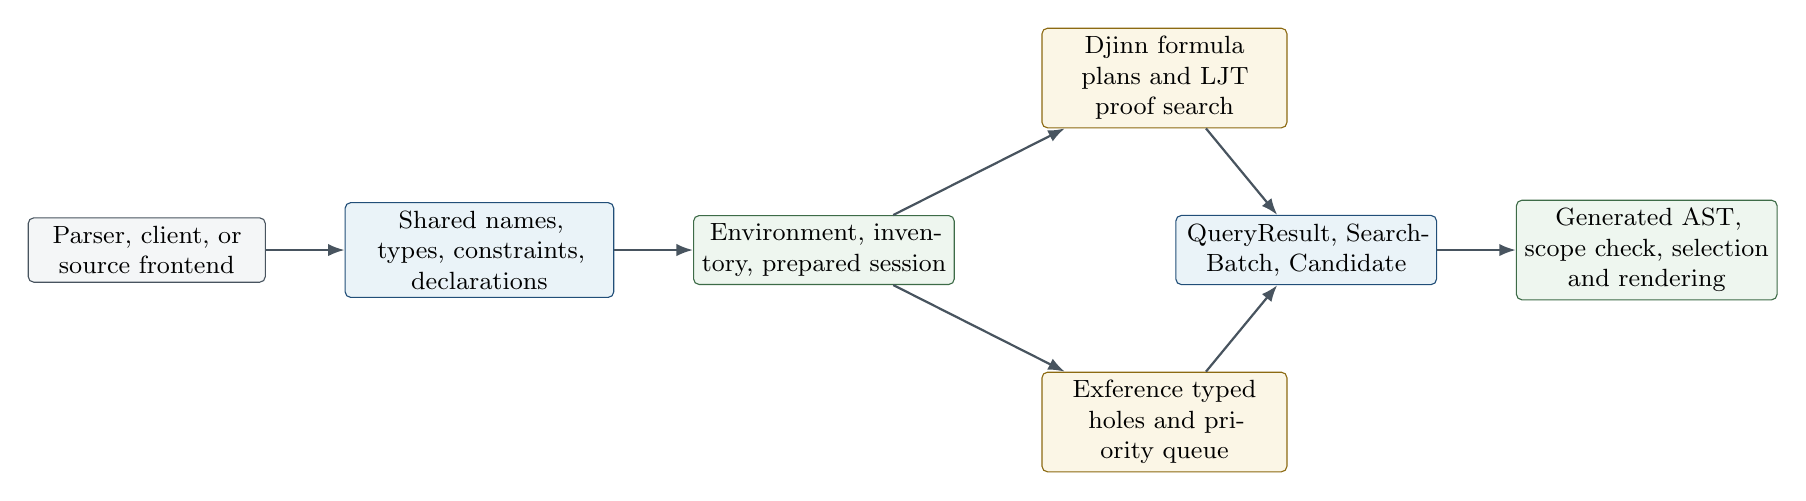
\begin{tikzpicture}[node distance=9mm and 10mm]
  \node[graybox,text width=28mm] (source) {Parser, client, or source frontend};
  \node[box,right=of source,text width=32mm] (vocab) {Shared names, types, constraints, declarations};
  \node[greenbox,right=of vocab,text width=31mm] (authority) {Environment, inventory, prepared session};
  \node[goldbox,above right=11mm and 11mm of authority,text width=29mm] (djinn) {Djinn formula plans and LJT proof search};
  \node[goldbox,below right=11mm and 11mm of authority,text width=29mm] (exf) {Exference typed holes and priority queue};
  \node[box,right=28mm of authority,text width=31mm] (result) {QueryResult, SearchBatch, Candidate};
  \node[greenbox,right=of result,text width=31mm] (generated) {Generated AST, scope check, selection and rendering};

  \draw[flow] (source) -- (vocab);
  \draw[flow] (vocab) -- (authority);
  \draw[flow] (authority) -- (djinn);
  \draw[flow] (authority) -- (exf);
  \draw[flow] (djinn) -- (result);
  \draw[flow] (exf) -- (result);
  \draw[flow] (result) -- (generated);
\end{tikzpicture}}
\caption{Djex's ownership flow. Both engines consume projections derived from one checked source authority and return values in one checked result and generated-code vocabulary.}
\label{fig:djex-runtime}
\end{figure}

\section{The representation ladder}

A request crosses several representations. Each transition either validates information, deliberately hides information, or derives an engine-specific cache.

\begin{longtable}{@{}L{0.20\textwidth}L{0.27\textwidth}L{0.45\textwidth}@{}}
\toprule
\textbf{Representation} & \textbf{Owner} & \textbf{Purpose and information content} \\
\midrule
\endhead
Source syntax or client AST & Frontend/client & User spelling, parser locations, imports, module qualification, and possibly language-specific structure. It is not yet a synthesis authority. \\
Shared source vocabulary & \filepath{Language.Haskell.Synthesis.*} & Validated names, kinds, types, constraints, declarations, qualification policy, and generated-definition names. \\
\code{Environment} & Shared foundation & One declaration stream sealed together with coherent indexes and namespace ownership. Hidden construction prevents the indexes from drifting. \\
\code{Inventory}/prepared inventory & Shared foundation & The environment paired with inferred kind assumptions, exact synonym tables, class views, and transient lowering projections. \\
Backend session & Djinn or Exference adapter & Immutable backend-specific indexes derived from the same prepared inventory, plus explicit omission or capability metadata. \\
Checked request & Backend adapter & An opaque request whose target, goal, contexts, options, provenance, width bounds, and session-dependent elaboration have crossed the appropriate validation phases. \\
Backend search state & Djinn or Exference core & Djinn formulas, proof environments, proof streams, and plan families; or Exference typed holes, scopes, substitutions, constraints, usage counters, and rated queue nodes. \\
Shared result envelope & Query/search/candidate modules & Logical evidence, progress/completion, metadata, residual constraints, and backend-owned candidate details without erasing backend distinctions. \\
Generated syntax & \code{Generated} and renderers & Scoped expressions, patterns, clauses, visible type applications, simplification, alpha-equivalence, local-name allocation, and Haskell rendering. \\
\bottomrule
\end{longtable}

The design rule is simple but strict: a later representation may use only information explicitly retained by an earlier one. A rendered forall spelling is not a logical identity; an alpha-normal \code{TypeAtom} key is. A candidate score is not evidence; a checked proof or reconstructed expression is. A finished heuristic search is not a refutation.

\section{Checked authorities}

Several central types have hidden constructors because their representation itself carries a proof obligation.

\begin{itemize}
  \item \code{Environment} certifies that declaration order and every type, value, constructor, class, instance, and occupied-name index agree.
  \item Prepared inventories certify kind assumptions and synonym meaning for one exact environment.
  \item Djinn and Exference sessions certify that backend projections were produced from that authority under one explicit policy.
  \item Checked requests certify that target naming, structural bounds, source provenance, and session-dependent elaboration were performed in the documented order.
  \item \code{DefinitionName}, \code{VisibleTypeArgument}, and other small opaque wrappers prevent invalid generated syntax from entering the common AST.
\end{itemize}

A recurring implementation convention follows from this: invariant-bearing observations are ordinary functions rather than exported record fields when record update would let a caller bypass a smart constructor. Opaque authorities also avoid deriving \code{Generic} when \code{GHC.Generics.to} could forge a supposedly checked value.

\begin{invariantbox}
A backend cache is never an alternative source of truth. Replacing declarations means constructing and sealing a replacement environment/session, not editing a private index and hoping the shared view still agrees.
\end{invariantbox}

\section{Evidence and progress are independent}

Djex deliberately models two questions separately:

\begin{enumerate}
  \item \emph{What logical fact, if any, did the backend establish?}
  \item \emph{Did the configured operational exploration finish, continue, or stop at a bound?}
\end{enumerate}

A search may return validated candidates and still be truncated. Djinn may exhaust an incomplete formula plan and therefore have no sound negative claim. Exference may empty its queue after exploring every retained node but still supply only \code{NoEvidence}. Conversely, a complete unbudgeted Djinn search may return \code{ProvedUninhabitable} together with ordinary \code{Finished} progress.

The semantic stratum adds a third independent axis: \emph{behavioral association}. \dpath{synthesis/src/Language/Haskell/Synthesis/Semantic/Problem.hs} binds a raw solver or behavioral observation to exact inventory, encoding, candidate, and problem fingerprints, and its design rule is explicit: ``Association is not certification. Every raw solver or behavioral result, including \code{unsat}, is exposed as \code{HeuristicRankingOnly}.'' An associated solver verdict may rank candidates, but it becomes \code{BehavioralEvidence} only through independent domain replay against the exact query problem. This is the same discipline as the existing rule that a finished heuristic search is not a refutation, extended to external solvers.

\begin{center}
\begin{tabularx}{0.94\textwidth}{@{}L{0.26\textwidth}L{0.28\textwidth}Y@{}}
\toprule
\textbf{Observation} & \textbf{Meaning} & \textbf{What it does not mean} \\
\midrule
\code{ValidatedCandidates} & At least one backend candidate passed the backend's independent result boundary. & The search explored every alternative. \\
\code{ProvedUninhabitable} & Djinn proved the accepted translated problem has no inhabitant under a complete, exhaustive plan. & Every richer source language embedding is also impossible. \\
\code{RequiresTargetReference} & The only proof found after diagnostic reintroduction uses the target being defined. & General recursion is silently acceptable. \\
\code{NoEvidence} with \code{Finished} & The configured exploration ended without a logical claim. & The type is uninhabited. \\
\code{Truncated reasons} & Unexplored work may remain for the listed operational reasons. & Already returned candidates are invalid. \\
\code{HeuristicRankingOnly} & A solver or behavioral observation, including \code{unsat}, was associated with an exact fingerprinted problem. & The observation certifies anything; only independent replay creates \code{BehavioralEvidence}. \\
\bottomrule
\end{tabularx}
\end{center}

\section{The semantic stratum}\label{sec:semantic-stratum}

The newest stratum gives candidates a checked \emph{behavioral} story alongside their typing story. It is backend-neutral, lives in \filepath{synthesis/src} with package-private internals in \filepath{synthesis/internal}, and is re-exported from the facade.

\textbf{Length contracts.} \dpath{synthesis/src/Language/Haskell/Synthesis/Semantic/Length.hs} defines the \code{finite-list-spine-length/v1} dialect---total finite list-spine lengths over unbounded naturals with opaque payloads---and its distinct \code{finite-binary-product-spine-lengths/v1} sibling, whose exact boxed binary product relates either result component to the modeled inputs. Provider summaries are explicit assumed laws for search guidance, never behavioral evidence.

\textbf{The SMT-LIB/Z3 live stack.} \dpath{synthesis/src/Language/Haskell/Synthesis/Semantic/Length/SMTLib/Live.hs} owns one capability-probed Z3 worker for the dynamic extent of a lexical scope; one scope admits 64 scalar-plus-product transactions in total, not 64 of each. Failures are sanitized: callers can observe status and heuristic strength, but no process handle, executable or workspace path, transcript, or run identity crosses the facade. Solver status remains an observation---\code{unsat} is relative to the checked encoding and is restricted to \code{HeuristicRankingOnly}. The pure framing and phase control shared by both query shapes is one protocol machine in \dpath{synthesis/internal/Language/Haskell/Synthesis/Internal/Semantic/Length/SMTLib/Protocol.hs}, parameterized by a \code{LengthSMTLibProtocolIdentity} record carrying schema tags, fingerprint roles, and query projections; \code{Protocol.SpinePair} is a thin wrapper contributing only what distinguishes the product domain.

\textbf{Typed candidates, certificates, and fingerprints.} A \code{Fingerprint} is the complete versioned canonical encoding of an identity, not a lossy hash, with package-private construction. \code{TypedCandidate} and \code{TypedGenerated} retain a bounded typed term graph beside the historical candidate syntax, and the package-private certificate table proves bounded capture-avoiding replay of one complete leading forall telescope; graph association is atomic against exact inventory, encoding, candidate, and problem fingerprints. Throughout the stratum only independent replay creates evidence---association, solver output, and certificates alone certify nothing.

For the chronological engineering record behind this stratum, see \dpath{docs/reports/README.md}; the module Haddock carries the per-boundary detail.

\section{Backend contrast}

\begin{longtable}{@{}L{0.21\textwidth}L{0.34\textwidth}L{0.37\textwidth}@{}}
\toprule
\textbf{Dimension} & \textbf{Djinn} & \textbf{Exference} \\
\midrule
\endhead
Core model & Intuitionistic formula compilation and contraction-free LJT proof search. & Priority-ordered typed-hole search with unification, constraints, scopes, and heuristic penalties. \\
Primary output & Proof-derived generated clauses, usually closed and constraint-free. & Ranked generated clauses with metrics and possibly residual constraints. \\
Negative evidence & Possible when translation is complete and search is exhaustive and unbudgeted. & Never claimed by the adapter. \\
Rank-N policy & Positive introduction plus opaque alpha-aware atoms, bounded complementary formula plans, and controlled instantiation axioms. & Positive introduction, local elimination, opaque polytype atoms in unification, rigid scope tracking, and visible type application. \\
Class constraints & Validated, but ordinary inhabitation remains dictionary-independent. & Resolved through query/static class environments; residuals may be retained by policy. \\
Independent checker & LJT proof checker before proof lowering. & Bidirectional expression checker that reconstructs the final candidate without trusting the search node. \\
Search controls & Alternatives, depth-first/interleaved strategy, candidate cutoff, optional choice-point budget. & Step, queue, depth, constraint-deferral, pattern, unused-binder, residual-constraint, and heuristic controls. \\
\bottomrule
\end{longtable}

\section{Cross-cutting invariants}

The same engineering principles recur throughout the repository:

\begin{itemize}
  \item source order is retained explicitly for diagnostics, declarations, constraints, candidates, and duplicate reporting;
  \item arbitrary-precision counts are used until an established compatibility surface requires a bounded \code{Int};
  \item potentially cyclic caller-built lists and trees are observed through explicit bounds before their elements are entered;
  \item substitution is capture-avoiding and binder-aware, with deterministic allocation and explicit exhaustion;
  \item alpha identity is structural and lexical, never reconstructed from rendered text;
  \item search laziness is part of the contract: selectors and result constructors avoid forcing uninspected candidate tails;
  \item every engine proposal crosses an independent checker before it becomes a canonical candidate;
  \item compatibility APIs remain available, but stable adapters keep checked source authority and backend caches inseparable.
\end{itemize}

\begin{sourcebox}
Start with \dpath{docs/architecture.md}, \dpath{synthesis/README.md}, and \dpath{src/Language/Haskell/Djex.hs}. Then follow one backend through its stable adapter into its core rather than entering an \code{Internal} module without the request/session context that establishes its invariants.
\end{sourcebox}

\chapter{One synthesis request, end to end}\label{ch:djex-query-lifecycle}

Consider the polymorphic application type
\[
  \forall a\,b.\;(a \to b) \to a \to b.
\]
This chapter traces a native shared request rather than a parser-specific compatibility request.

\section{Stage 1: construct the shared goal}

A client first constructs checked names and a shared type tree. Schematic code looks like this:

\begin{lstlisting}[language=Haskellish]
a = "a"
b = "b"
goal = ForallType [a, b] []
         (FunctionType
           (FunctionType (TypeVariable a) (TypeVariable b))
           (FunctionType (TypeVariable a) (TypeVariable b)))
\end{lstlisting}

Actual public code obtains structural names through the checked \code{Name} constructors and the target through \code{mkDefinitionName}. The shared type boundary validates tuple widths, constructor positions, forall binders, constraint names, and canonical function/tuple representation before a backend may depend on the shape.

\section{Stage 2: seal the declaration authority}

Declarations are passed to \code{mkEnvironment}. The constructor validates each declaration in source order, preflights known class arities before entering lazy argument spines, and inserts it transactionally into every relevant index. Kind inference then produces an \code{Inventory}; exact type-synonym preparation keeps the original environment and its normalized synonym table inseparable.

A backend session derives its private search projection once. The Djinn session caches formula compilers, premise projections, recursive classifications, class arities, and prepared environment data. The Exference session lowers supported declarations to functions, deconstructors, classes, exact schemes, rigid-instantiation context, and omission diagnostics. Neither session exposes mutable caches.

\section{Stage 3: seal the request}

The neutral request contains a checked target, goal, explicit contexts, and backend-specific options:

\begin{lstlisting}[language=Haskellish]
QueryRequest
  { requestTarget   = target
  , requestGoal     = goal
  , requestContexts = []
  , requestOptions  = options
  }
\end{lstlisting}

\code{mkDjinnRequest} and \code{mkExferenceRequest} create different opaque request types. Session-independent preflight happens at construction; session-owned checks---known class widths, synonym elaboration, joint kind scope, exact scheme lookup, or backend lowering---happen when the request runs against a session. This split allows a checked request to be reused against another compatible session without smuggling one session's alias meanings into another.

\section{Stage 4A: Djinn preparation and formula plans}

Djinn inserts explicit request contexts beneath the leading forall chain, bounds every context argument before full traversal, and implicitizes the prenex binders with fresh variables. Contexts remain validation obligations; class methods do not become monomorphic proof premises.

The prepared formula compiler expands aliases, finite datatypes, abstract types, and bounded recursive structure under polarity-aware rules. Positive supported foralls may be opened with fresh skolems. Unsupported or negative occurrences remain alpha-aware opaque propositions. The compiler emits a primary opened plan, an exact opaque plan, and bounded complementary frontiers. Each plan records whether its translation is incomplete.

For the example the logical core is
\[
  (A \to B) \to A \to B.
\]
LJT introduces both assumptions and applies the first to the second. The raw proof is checked against the exact formula and proof environment, then lowered to a shared generated clause equivalent to:

\begin{lstlisting}[language=Haskellish]
Lambda [Bind "f", Bind "x"]
  (Apply (Local "f") (Local "x"))
\end{lstlisting}

Only a complete plan whose unbudgeted search exhausts every branch may produce negative evidence. Candidate-producing incomplete plans remain useful because every returned proof is checked against the formula that generated it.

\section{Stage 4B: Exference preparation and typed-hole search}

Exference validates options before source-provenance-dependent work, elaborates the goal in the exact session synonym/kind scope, lowers it to the native shared/Exference type, and prepares a rigid-instantiation plan for the leading foralls.

The root node contains one hole whose expected type is the instantiated goal. Opening the arrow chain adds \code{f : A -> B} and \code{x : A} to a checked lexical scope. Selecting \code{f} for the result hole creates an argument hole of type \code{A}; selecting \code{x} fills it. Each branch carries substitutions, scoped constraints, rigid provenance, variable-usage counts, remaining goals, and a heuristic depth.

A solved node is simplified and then passed to the independent expression checker. The checker reconstructs the type from the final expression, environment, exact schemes, class context, and rigid plan. It does not trust the search node's conclusion. Only checked outputs are projected to the common generated AST and result envelope.

\section{Stage 5: package the result}

Both adapters return \code{QueryResult metadata candidate}. A result contains:

\begin{itemize}
  \item logical \code{QueryEvidence};
  \item one \code{SearchBatch} with progress, metadata, and candidate list, or a lazy trace of such batches;
  \item backend-specific candidate details, such as Djinn's unused-binder score or Exference's step/complexity/queue metrics;
  \item shared generated output and residual constraints.
\end{itemize}

The smart result constructor checks evidence/candidate consistency without forcing an uninspected candidate tail. Frontends may then use \code{Selection} policies to take the first result, best score, bounded lookahead, all results, or preferred tiers while preserving the strongest progress actually observed.

\section{Stage 6: render without weakening the boundary}

Rendering is not a raw \code{Show}. The shared renderer checks scope and syntax, allocates collision-free local names, applies a qualification policy, and handles visible type applications, tuples, lets, cases, patterns, and top-level clauses. Djinn additionally rejects forged residual constraints because genuine Djinn candidates are closed. Exference validates caller-built residual constraints and supplies deterministic fallback type-variable names when hint maps are malformed, oversized, partial, or cyclic.

For the example, the candidate definition is morally:

\begin{lstlisting}[language=Haskellish]
apply f x = f x
\end{lstlisting}

The exact spelling depends on the checked target, local-name hints, and qualification policy; the semantic output remains the shared \code{FunctionClause}.

\section{Provider-local instantiation evidence}

A richer client may also supply external evidence for exact polymorphic providers. Djex exposes three levels:

\begin{itemize}
  \item \code{ProviderInstantiationCandidate}: one closed proper-type choice for an exact provider;
  \item \code{ProviderInstantiationAssignment}: one complete ordered vector for all leading binders;
  \item \code{KindedProviderInstantiationAssignment}: the same vector paired with exact ground kinds.
\end{itemize}

The adapters bound the outer list and every argument vector before entering caller values. They verify that the provider exists in the exact session, that arity and kinds match its retained scheme, that arguments are closed and otherwise admissible, and that alpha-equivalent duplicates are removed per provider. The vector remains correlated throughout search; it is never reconstructed from an accidental Cartesian product of independent argument pools.

\section{Failure ordering is part of the API}

The code deliberately chooses which failure is observed first. Examples include:

\begin{itemize}
  \item target-name validation before parsing a textual Djinn request;
  \item option validation before session-dependent Exference elaboration;
  \item known class arity before traversing a possibly cyclic argument spine;
  \item synonym saturation before later structural/kind diagnostics;
  \item generated scope/syntax failure before Djinn's forged-residual check;
  \item ordinary query validation before optional provider evidence.
\end{itemize}

These precedence rules are not cosmetic. They make diagnostics deterministic, prevent a later malformed value from hiding an earlier structural failure, and ensure that cyclic compatibility values fail finitely rather than changing which semantic error a caller observes.

\begin{summarybox}
A Djex request is not handed directly to a search function. It moves through checked source vocabulary, a sealed environment and inventory, an immutable backend session, an opaque request, backend-specific preparation, independent proof/expression checking, the shared result envelope, and finally generated-syntax validation and rendering.
\end{summarybox}

\part{Detailed codebase walkthrough}

\chapter{Repository, package, and module map}\label{ch:djex-map}

\section{The package is one component with several source roots}

The top-level \dpath{djex.cabal} describes one package that deliberately preserves several historical trees while exposing a converged library. The important source roots are:

\begin{longtable}{@{}L{0.24\textwidth}L{0.68\textwidth}@{}}
\toprule
\textbf{Root} & \textbf{Responsibility} \\
\midrule
\endhead
\filepath{synthesis/src} & Shared synthesis vocabulary and validation: names, kinds, types, type atoms, constraints, declarations, environments, inventories, kind inference, queries, search progress, candidates, generated terms, diagnostics, selection, and rendering helpers. Also the public semantic surface: Length contracts, the SMT-LIB/Z3 boundary, typed candidates, and fingerprints. \\
\filepath{synthesis/internal} & Package-private home modules behind the semantic surface: fingerprint representation, type-application certificates, class resolution, and the Length/SMT-LIB/Z3 protocol, session, and execution internals. Compiled into the library but exposed to no public importer. \\
\filepath{djinn/src-core} & Djinn's checked adapter, session/request internals, type-to-formula compiler, LJT proof search, proof checker, instantiation machinery, and proof-to-generated lowering. \\
\filepath{djinn/src-internal} & Package-private Djinn support modules: \code{CheckedCandidate}, \code{GeneratedDeduplication}, \code{InstantiationEvidence}, and \code{ProofCheck.Evidence}. \\
\filepath{djinn/src-frontend} & Historical Djinn-compatible API and REPL facade. It is important for compatibility, but it should not own shared invariants. \\
\filepath{exference/src-core} & Exference's checked adapter and its engine: unification, class constraints, typed expression, typed holes, scopes, queue scheduler, scoring, rigid instantiation, independent expression checker, and diagnostics. \\
\filepath{exference/src-frontend} & Historical Exference source parser, environment loader, Haskell conversion layer, and CLI. \\
\filepath{src} & Unified Djex facade, unified command line and REPL, package/workspace handling, source translation, and the small public entry surface used by new clients. \\
\bottomrule
\end{longtable}

The library compiles exactly these eight source roots; \filepath{synthesis/internal} and \filepath{djinn/src-internal} carry only package-private home modules. A ninth directory, \filepath{test-support/}, is not part of the library: it holds the shared \code{CLIAssertions} test module and the two private fixture executables described below.

The Cabal file also exposes historical \code{djinn} and \code{exference} executables alongside \code{djex}, and builds two private test fixtures, \code{djex-fake-cabal} and \code{djex-fake-z3}. This is not merely packaging clutter. It lets the project maintain compatibility tests while moving semantic ownership into shared modules, and it lets process-launching behavior be tested against controlled stand-ins.

\begin{figure}[htbp]
\centering
\resizebox{0.97\textwidth}{!}{%
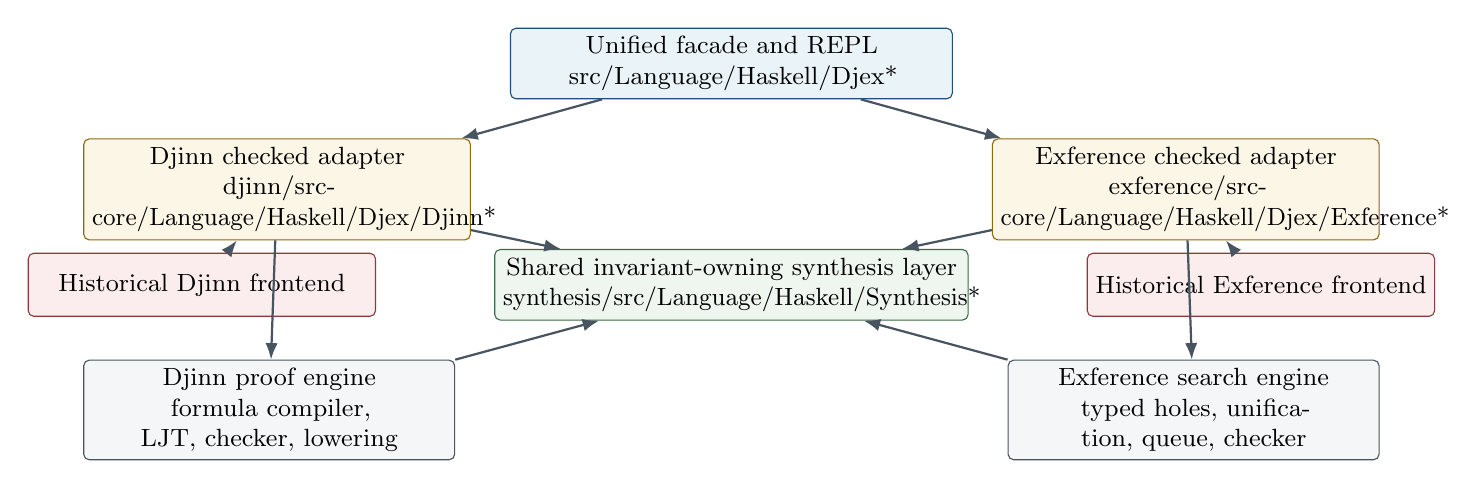
\begin{tikzpicture}[node distance=7mm]
  \node[box,text width=54mm] (facade) {Unified facade and REPL\\\filepath{src/Language/Haskell/Djex*}};
  \node[goldbox,below left=of facade,text width=47mm] (dadapter) {Djinn checked adapter\\\filepath{djinn/src-core/Language/Haskell/Djex/Djinn*}};
  \node[goldbox,below right=of facade,text width=47mm] (eadapter) {Exference checked adapter\\\filepath{exference/src-core/Language/Haskell/Djex/Exference*}};
  \node[greenbox,below=19mm of facade,text width=58mm] (shared) {Shared invariant-owning synthesis layer\\\filepath{synthesis/src/Language/Haskell/Synthesis*}};
  \node[graybox,below left=of shared,text width=45mm] (djinn) {Djinn proof engine\\formula compiler, LJT, checker, lowering};
  \node[graybox,below right=of shared,text width=45mm] (exf) {Exference search engine\\typed holes, unification, queue, checker};
  \node[redbox,left=15mm of shared,text width=42mm] (oldD) {Historical Djinn frontend};
  \node[redbox,right=15mm of shared,text width=42mm] (oldE) {Historical Exference frontend};

  \draw[flow] (facade) -- (dadapter);
  \draw[flow] (facade) -- (eadapter);
  \draw[flow] (dadapter) -- (shared);
  \draw[flow] (eadapter) -- (shared);
  \draw[flow] (dadapter) -- (djinn);
  \draw[flow] (eadapter) -- (exf);
  \draw[flow] (djinn) -- (shared);
  \draw[flow] (exf) -- (shared);
  \draw[flow] (oldD) -- (dadapter);
  \draw[flow] (oldE) -- (eadapter);
\end{tikzpicture}}
\caption{Djex's dependency intent. Shared semantic types sit below the adapters; backend-specific search remains sealed. The historical frontends point inward rather than defining new semantic authorities.}
\label{fig:djex-layers}
\end{figure}

\section{The central architectural rule}

The package converges infrastructure without pretending the engines are the same algorithm. Shared modules own contracts that both engines must honor. The adapters own conversion and backend policy. Djinn and Exference retain distinct search representations, ordering, completeness properties, and diagnostics.

This rule explains many otherwise surprising boundaries:

\begin{itemize}
  \item The shared \code{Type} is rich enough for both engines, but neither backend is forced to inspect every constructor identically.
  \item The shared \code{Generated} AST is a target language, but each backend may reach it by a different checked route.
  \item Search progress is shared, but the meaning of queue exhaustion differs from proof-search exhaustion.
  \item Provider-instantiation assignments are shared evidence, but each backend validates and consumes them in its own request preparation.
  \item The facade can expose a capability matrix instead of lying that every backend has every property.
\end{itemize}

\begin{designbox}
A tempting unification would be one giant \code{SearchState} and one generic step function parameterized by callbacks. That would erase exactly the information that makes the engines valuable: Djinn's proof-theoretic completeness story and Exference's ranking, type-directed expansion, and source-oriented heuristics. Djex instead unifies the borders and leaves the centers different.
\end{designbox}

\section{Recommended first reading order}

For a new maintainer, the shortest path to a correct mental model is:

\begin{enumerate}
  \item \dpath{synthesis/README.md} for the shared contract;
  \item \dpath{synthesis/src/Language/Haskell/Synthesis/Type.hs}, then \dpath{synthesis/src/Language/Haskell/Synthesis/Environment.hs};
  \item \dpath{synthesis/src/Language/Haskell/Synthesis/Query.hs}, \dpath{synthesis/src/Language/Haskell/Synthesis/Search.hs}, and \dpath{synthesis/src/Language/Haskell/Synthesis/Generated.hs};
  \item \dpath{djinn/src-core/Language/Haskell/Djex/Djinn.hs} and \dpath{djinn/src-core/Djinn/Core.hs};
  \item \dpath{exference/src-core/Language/Haskell/Djex/Exference.hs} and \dpath{exference/src-core/Language/Haskell/Exference/Core/Internal/Exference.hs};
  \item \dpath{src/Language/Haskell/Djex.hs} and the unified REPL modules.
\end{enumerate}

Do not start by reading the two largest backend files linearly. First learn what their inputs and outputs are permitted to mean. Otherwise implementation details such as freshness supplies, proof-plan families, or queue pruning have no frame of reference.

\chapter{The shared synthesis foundation}\label{ch:djex-shared}

\section{Names are checked data, not strings}

The shared name layer in \dpath{synthesis/src/Language/Haskell/Synthesis/Name.hs} distinguishes namespaces and syntactic roles. Values such as identifiers, type constructor names, data constructor names, class names, method names, and definition names are not freely interchangeable. Smart constructors validate spellings and reserved forms; rendering can therefore rely on the distinction without reparsing arbitrary text.

This is a small example of the project's general style: validate once, hide the constructor, and pass an authority value downward. A backend should not have to ask repeatedly whether the query target is a legal definition name.

The layer also separates semantic identity from qualification and source spelling. That matters because a generated term may need a fully qualified source name even though environment lookup used a canonical key, and because a local binder must never be confused with a global declaration merely because the text matches.

\section{Kinds and the neutral type language}

The neutral type language is centered in \dpath{synthesis/src/Language/Haskell/Synthesis/Type.hs}. At a high level it contains:

\begin{lstlisting}[language=Haskellish]
data Variable id
  = FlexibleVariable id
  | RigidVariable id

data Type v
  = TypeVariable v
  | TypeConstructor Name
  | TypeApplication (Type v) (Type v)
  | FunctionType (Type v) (Type v)
  | TupleType Boxity [Type v]
  | ForallType [v] [Constraint (Type v)] (Type v)
\end{lstlisting}

The precise exported surface is richer, but this sketch captures the semantic split. Flexible variables are unification variables in Exference and instantiation variables in shared validation. Rigid variables are constants scoped by a binder or exact assignment. A forall stores its binders and class constraints explicitly. Tuples retain boxity and arity rather than being flattened to anonymous constructor applications at the public boundary.

\subsection{Canonical forms without erasing source distinctions}

The module provides canonical function and tuple views, strict application and function spines, constructor-application views for higher-kinded unification, free-variable and binder analysis, global binder renaming, and capture-avoiding simultaneous substitution.

The important qualification is \emph{without erasing source distinctions}. Normalization may turn a saturated representation into a canonical form for comparison, but it must not dissolve a nested polytype into ordinary first-order nodes or forget that a nominal constructor came from a particular source declaration.

For example, higher-kinded unification wants to observe
\[
  F\;a\;b
\]
as a head plus arguments, and it wants functions and tuples to participate in the same application machinery. That is the purpose of a constructor-application view. It is not permission to rewrite every type permanently into an untyped list of symbols.

\subsection{Finite observation boundaries}

Many public values are Haskell lists, and clients can accidentally supply cyclic or infinite lists. Constructors that must establish a finite invariant do not blindly call \code{length}. They observe only a documented maximum width plus a sentinel element, then reject oversize or nonterminating shapes at a bounded frontier where possible. The same principle appears in provider assignment vectors, class arities, kind trees, generated hints, and search prefixes.

\begin{invariantbox}
Strict authorities never retain a value whose validity depends on consuming an unbounded lazy tail. Laziness is reserved for search result streams and other places where incremental observation is itself the API.
\end{invariantbox}

\section{Type atoms: opaque, alpha-aware islands}

\dpath{synthesis/src/Language/Haskell/Synthesis/TypeAtom.hs} solves a particularly difficult problem. A nested polymorphic type can be meaningful as a whole without being safe to decompose in a first-order unifier. Djex therefore represents such a region as a \code{TypeAtom}: an exact source tree paired with an alpha-normal lexical key and enough variable information for substitution and occurs checks.

Ordinary unification treats the atom as opaque. Equality remains alpha-aware. Free variables inside the atom still participate in capture avoidance and occurs checks. Thus Djex avoids two unsound extremes:

\begin{itemize}
  \item treating the atom as a completely uninterpreted string, which would lose alpha-equivalence and variable provenance;
  \item opening the atom as if rank-N structure were ordinary first-order syntax, which would allow invalid decomposition and escaping binders.
\end{itemize}

Type atoms recur in both backends. Djinn may compile a nested negative forall to an opaque proposition symbol keyed by a type atom. Exference's unifier may bind an opaque polytype as one unit but cannot descend into it.

\section{Constraints, classes, declarations, and synonyms}

The shared declaration vocabulary spans \dpath{synthesis/src/Language/Haskell/Synthesis/Constraint.hs}, \dpath{synthesis/src/Language/Haskell/Synthesis/Class.hs}, \dpath{synthesis/src/Language/Haskell/Synthesis/Declaration.hs}, and \dpath{synthesis/src/Language/Haskell/Synthesis/TypeSynonym.hs}. It models value signatures, data/type declarations, classes, instances, methods, constraints, and type synonyms in source order.

Source order is significant. A declaration can only refer to authorities already established by the prefix unless a specific recursive form permits otherwise. Type-synonym expansion must terminate or report a cycle. Class validation must know arity, superclass prerequisites, method ownership, and instance-head shape. Those checks belong before either backend builds a session.

The shared kind inference module, \dpath{synthesis/src/Language/Haskell/Synthesis/KindInference.hs}, validates type applications and exact provider assignments across proper and higher kinds. This is why provider evidence carries kind information rather than a flat list of types.

\section{Environment as an authority}\label{sec:djex-environment}

\dpath{synthesis/src/Language/Haskell/Synthesis/Environment.hs} is one of the most important files in the repository. The public \code{Environment} is opaque. Internally it retains the source declarations and several strict indexes: types, values, constructors, classes, instances, instance heads, and occupied names. \code{mkEnvironment} validates the entire declaration sequence before constructing those indexes.

The indexes are duplicated views of one semantic state. An update must therefore be transactional: either the declaration and all relevant indexes advance together, or the old environment remains. Code that appends a declaration to the source list but forgets an instance-head index would create an internally contradictory authority.

A useful way to read the constructor is as a fold over declarations with a large invariant:

\begin{lstlisting}[language=Haskellish]
step :: CheckedPrefix -> Declaration -> Either Diagnostic CheckedPrefix
step prefix declaration = do
  validateNamespaces prefix declaration
  validateKinds      prefix declaration
  validateClasses    prefix declaration
  validateInstances  prefix declaration
  updateEveryIndex   prefix declaration
\end{lstlisting}

This is explanatory pseudocode, not a literal excerpt. The actual code has more specialized paths, but the transactional model is accurate.

\subsection{Inventory and prepared inventory}

\dpath{synthesis/src/Language/Haskell/Synthesis/Inventory.hs} derives a search-oriented inventory from the environment. A prepared inventory is another opaque authority: aliases are expanded where permitted, recursive components are classified, and lookup tables are normalized for backend consumption.

The project also distinguishes a transient \emph{prepared-inventory expansion}. That view may expose alias-free structures and recursion metadata for a particular operation, but it is not retained as a long-lived authority. This prevents a temporary expansion policy from silently becoming the canonical meaning of the environment.

\begin{designbox}
The environment answers, ``What declarations exist and are they coherent?'' The inventory answers, ``What search-facing facts can be derived from that environment?'' A prepared expansion answers, ``What does this particular type look like after this bounded expansion policy?'' Keeping these questions in separate types prevents a backend convenience from mutating source semantics.
\end{designbox}

\section{Queries and checked requests}

The public query language in \dpath{synthesis/src/Language/Haskell/Synthesis/Query.hs} contains a target definition name, a goal type, explicit contexts, and backend options. Provenance and display metadata may accompany the query, but semantic equality does not accidentally depend on incidental diagnostics.

A \code{CachedQuery} is opaque. It represents the result of normalization and validation that can safely be reused. The backend adapters then add session-specific checks and wrap it in private \code{DjinnRequest} or \code{ExferenceRequest} types. This two-stage preparation has a practical payoff: malformed shape is rejected once, while environment-dependent facts are checked against the exact session that will execute the query.

Provider evidence is part of the request contract. The shared forms distinguish:

\begin{itemize}
  \item a provider-instantiation candidate, describing a possible relation between a provider and a query occurrence;
  \item an assignment, choosing concrete arguments for that provider;
  \item a kinded assignment, retaining each argument's kind and exact representation.
\end{itemize}

The vectors are bounded. At this snapshot, a provider assignment supports at most six arguments, with finite caps on candidates and assignments. These limits are not merely performance knobs; they are part of the validation boundary that keeps exact evidence inspectable.

\section{Search progress and evidence}

\dpath{synthesis/src/Language/Haskell/Synthesis/Search.hs} defines backend-neutral progress. Truncation reasons include step and choice-point limits, candidate cutoffs, identifier exhaustion, queue pruning, and depth pruning. A batch can be continuing or completed; completion can be finished or truncated with one or more exact reasons.

The evidence layer remains backend-specific enough to be honest. Djinn can return validated candidates, a proof of uninhabitability for the translated problem, a self-reference-only diagnosis, or no evidence. Exference returns candidates and progress but never manufactures a negative proof from heuristic exhaustion.

\subsection{Candidate values}

\dpath{synthesis/src/Language/Haskell/Synthesis/Candidate.hs} packages a generated function clause with residual constraints and backend details. Backend details are intentionally extensible: Djinn can report proof/search information, while Exference can report steps, queue size, penalty, usage, and pruning statistics.

Candidate rendering revalidates scope. This may seem late, but it is a deliberate last defense before a neutral term crosses into source syntax. A candidate with an unbound local or an unresolved hole is not made printable merely because the search happened to construct it.

\section{The generated-term language}\label{sec:generated-ast}

The large \dpath{synthesis/src/Language/Haskell/Synthesis/Generated.hs} module is the common target of both backends. Its expression vocabulary includes locals, globals, holes during construction, application, visible type application, tuples, lambdas, lets, and cases. Patterns include binders, wildcards, tuples, declared constructors, and as-patterns. Function clauses associate checked definition names with expressions.

Several details are easy to miss:

\begin{itemize}
  \item \term{Visible type application} is a real AST node. It is not a string annotation. This lets exact rank-N instantiation evidence survive into rendering.
  \item Application-spine helpers are strict about mixed term and type arguments. They preserve order and do not silently commute them.
  \item Scope validation understands every binder-introducing pattern, including nested tuple and constructor patterns.
  \item Simplification is capture-aware and must preserve the source of global versus local names.
  \item Qualification is postponed until rendering, so semantic identity and source spelling remain separate.
\end{itemize}

\begin{invariantbox}
The shared generated AST is neither raw Haskell source nor a backend proof term. It is a checked intermediate language. Backend code may construct it; frontend code may render it; neither side may attach semantics by concatenating unvalidated strings.
\end{invariantbox}

\section{Diagnostics and selection}

\dpath{synthesis/src/Language/Haskell/Synthesis/Diagnostic.hs} gives validation and search failures structured identities and renderings. The adapters use diagnostics instead of throwing ordinary exceptions for expected user errors. Pure rendering paths still contain exception boundaries around hostile or infinite user-supplied text, but asynchronous exceptions are preserved.

\dpath{synthesis/src/Language/Haskell/Synthesis/Selection.hs} separates search generation from candidate selection. A backend may expose a lazy stream with scores and progress; a client chooses a bounded subset, filters it, and preserves the strongest progress observation. This is particularly important for any client that merges multiple lazy result streams or imposes its own bounded observation policy.

\begin{summarybox}
The shared layer establishes the vocabulary and the facts that both engines are allowed to assume. Its most important contribution is not code reuse but semantic compression: downstream code receives opaque values that stand for completed validation arguments.
\end{summarybox}

\chapter{Djinn: formulas, LJT proof search, and checked lowering}\label{ch:djinn}

\section{What Djinn promises}

Djinn is the proof-theoretic backend. It translates a supported type problem into intuitionistic propositional logic, searches for proof terms in a contraction-free LJT-style calculus, checks every proof independently, and lowers accepted proofs into the shared generated syntax. When translation is complete and search is genuinely exhaustive, failure can be negative evidence. That last property is the reason Djinn's request preparation, translation plans, and progress accounting are more elaborate than a simple ``type to formula'' function.

The stable adapter is \dpath{djinn/src-core/Language/Haskell/Djex/Djinn.hs}. Its private request and session support live in \dpath{djinn/src-core/Language/Haskell/Djex/Djinn/Internal/Request.hs} and \dpath{djinn/src-core/Language/Haskell/Djex/Djinn/Internal/Session.hs}. The major engine entry points are in \dpath{djinn/src-core/Djinn/Core.hs}.

\section{Request preparation}

Preparation occurs in two layers.

\subsection{Session-independent preflight}

The adapter first validates facts that do not depend on a loaded environment: the target definition name, goal width, binder shape, explicit context width, option bounds, and finite observations. This stage turns a public \code{QueryRequest} into a normalized cached query or a structured diagnostic.

The benefit is deterministic failure. A malformed query should not fail differently depending on which session happened to receive it, nor should it force a large environment before reporting a simple width error.

\subsection{Session-dependent elaboration}

The checked session supplies declarations, classes, constructor inventories, kind information, synonyms, and source names. The private request builder:

\begin{itemize}
  \item resolves and normalizes the goal against the prepared inventory;
  \item checks explicit class contexts against declared class arities;
  \item embeds contexts under the leading forall prefix in a representation that preserves scope;
  \item makes binder implicitness explicit to the compiler;
  \item verifies exact provider-instantiation assignments against the session;
  \item determines which loaded values and constructor schemas are eligible premises;
  \item excludes the target from the ordinary premise set.
\end{itemize}

Explicit contexts are validation obligations, not ordinary proof assumptions. A request for \code{C a => a -> a} should not be solved by treating the class dictionary as an arbitrary value of proposition \code{C a}; its role is to constrain the type and the admissible instances.

\begin{pitfallbox}
Reintroducing the target definition as a normal premise makes every recursive query trivially inhabitable. Djinn excludes it from the safe search environment. A separate diagnostic lane may reintroduce it only to establish that all observed proofs require self-reference.
\end{pitfallbox}

\section{The logical language}

\dpath{djinn/src-core/Djinn/Internal/LJTFormula.hs} defines the formula and proof-term vocabulary. In simplified form:

\begin{lstlisting}[language=Haskellish]
data Formula
  = Conj [Formula]
  | Disj [(ConsDesc, Formula)]
  | Empty Symbol
  | Formula :-> Formula
  | PVar Symbol

data Term
  = Var ... | Lam ... | Apply ...
  | Ctuple ... | Csplit ...
  | Cinj ... | Ccases ... | Xsel ...
\end{lstlisting}

Products become conjunctions; algebraic alternatives become labeled disjunctions; functions become implication; empty nominal types and opaque atoms become symbols. Constructor descriptions retain enough information for proof lowering to recover data-constructor applications and case alternatives.

\subsection{Symbols preserve nominal and opaque identity}

A symbol can be an ordinary logical name or an opaque type symbol paired with source information and a \code{TypeAtomKey}. This prevents two unrelated empty nominal types from collapsing merely because each has no visible constructor. It also ensures that alpha-equivalent opaque polytypes compare correctly while distinct nested polytypes remain distinct.

This is essential for sound negative evidence. If the compiler identified all opaque regions with one proposition, it could invent implications between unrelated source types. If it generated a fresh proposition for each occurrence, it would lose valid forwarding of the same opaque type. The key must therefore be semantic and alpha-aware.

\section{The prepared formula compiler}\label{sec:djinn-compiler}

\dpath{djinn/src-core/Djinn/Internal/TypeFormula.hs} is the bridge between the shared type authority and the proof calculus. It is best understood as a compiler producing both code and a proof obligation ledger.

A prepared compiler caches validated definitions, constructor descriptions, synonym expansions, and recursive-component classifications. A translation result contains at least:

\begin{itemize}
  \item the formula;
  \item whether the translation was incomplete;
  \item which positive forall sites were opened;
  \item which binders were skolemized;
  \item occurrence and origin metadata used to validate exact provider assignments;
  \item enough nominal information to lower a proof back to generated syntax.
\end{itemize}

\subsection{One-layer views}

The compiler does not recursively destruct every type by default. It uses a one-layer \code{TypeView}: observe the current constructor, decide whether that constructor is structurally admissible in the current polarity, and recursively compile only the selected children. This makes polarity and opacity policy explicit.

\subsection{Forall polarity}

A positive forall corresponds to producing a polymorphic value. Djinn can often open it by introducing a fresh rigid symbol. A negative forall corresponds to consuming a polymorphic value. Naively opening it would require impredicative or higher-rank reasoning beyond ordinary propositional translation. The conservative default is therefore:

\begin{itemize}
  \item open selected positive forall sites;
  \item preserve negative and unsupported nested sites as opaque type atoms;
  \item add exact instantiation axioms only when the request carries checked evidence.
\end{itemize}

This is why rank-N support appears as a family of translation plans rather than a single recursive function.

\subsection{Bounded plan families}

For a query with several openable sites, the compiler explores a deterministic family of structural plans:

\begin{itemize}
  \item all sites open;
  \item all sites opaque;
  \item selected singleton, pair, triple, quadruple, and quintuple frontiers in both open and opaque orientations;
  \item additional guarded plans tied to exact provider assignments and query-correlated closed instantiations.
\end{itemize}

The family is explicitly bounded. Quintuple combinations are capped per orientation, while remaining complete through a documented small number of sites. The cap is not hidden: if relevant plans were omitted, the translation carries incompleteness and a candidate-free search cannot become a refutation.

\begin{designbox}
Opening every positive forall is not always best. An opened site exposes structure that can enable a proof, but it can also destroy useful opaque equality: a value may simply need to be forwarded unchanged. The plan family searches both interpretations and deduplicates equivalent results afterward.
\end{designbox}

\subsection{Recursive and nominal data}

Recursive types require a similar duality. At a positive occurrence, the compiler may expose one constructor layer to synthesize or inspect data. At the same time it preserves an exact opaque fallback so forwarding remains possible without infinite unfolding. Recursive components are classified before compilation, and every exposure decision contributes to the completeness ledger.

Nominal parametric data is transported with constructor descriptions and parameter metadata. The compiler must not substitute a structurally similar but differently named type. Exact constructor identity is carried into proof terms and later lowering.

\subsection{Exact provider-assignment retention}

Provider assignments are only useful if the formula still represents the exact argument vector that was validated at the source boundary. The compiler records origins and occurrence paths and checks that a structural plan retains the assignment across aliases and higher-kinded application. A plan that has hidden or rearranged a relevant argument cannot consume the assignment merely because its pretty-printed formula looks compatible.

\section{LJT search}\label{sec:ljt-search}

The proof search implementation is in \dpath{djinn/src-core/Djinn/Internal/LJT.hs}. It combines a contraction-free sequent calculus with a continuation-encoded lazy search monad.

\subsection{Search modes}

A search mode chooses an exploration strategy and an optional global choice-point budget. The principal strategies are depth-first exploration and fair interleaving. The default unbudgeted mode is intended to retain the calculus's completeness properties, subject to documented local fairness adjustments.

The result stream is lazy. A client may consume the first proof without constructing every proof. At the same time, budget and exhaustion information remain observable. Internally, the search distinguishes:

\begin{itemize}
  \item a completed branch;
  \item a yielded proof with a continuation;
  \item an administrative step that advances the proof machine without producing a proof.
\end{itemize}

This distinction permits exact choice-point accounting and fair merges without forcing the whole tree.

\subsection{Antecedent classification}

LJT gains much of its behavior by classifying antecedents. The implementation separates pending formulas, atomic implications, nested implications, and already available atomic proofs. Right-reduction introduces functions, products, or disjunction choices. Left-reduction selects an assumption and applies the appropriate elimination rule.

The calculus is contraction-free in its structural formulation: it avoids arbitrary duplication as a primitive rule. Where a proof term must use an assumption more than once, the formula-specific left rule accounts for it. This keeps the search space much smaller than a naive natural-deduction enumerator.

\subsection{Cheap reachability pruning}

A necessary-condition test, conceptually \code{goalMayBeReachable}, rejects branches whose atomic goal symbols cannot arise from the current antecedents. This is not a theorem prover by itself; it is a conservative prune. Returning false must mean the branch is impossible. Returning true merely allows full proof search to continue.

\subsection{Fairness for repeated endomorphisms}

Types with several endomorphism assumptions can produce infinite local families such as \code{f x}, \code{f (f x)}, and so on. Pure depth-first exploration can starve sibling compositions. The implementation applies a local round-robin or interleaving policy for repeated binary endomorphism opportunities. Freshness and substitution machinery ensure that copied proof fragments do not capture binders.

\subsection{Normalization}

Proof terms are normalized before checking and lowering. The normalizer beta-reduces lambda applications, tuple split redexes, and case/injection redexes. Normalization reduces duplicate candidates and gives the proof checker a simpler object. It must remain binder-safe: every copied binder is freshened before substitution.

\begin{figure}[htbp]
\centering
\resizebox{0.96\textwidth}{!}{%
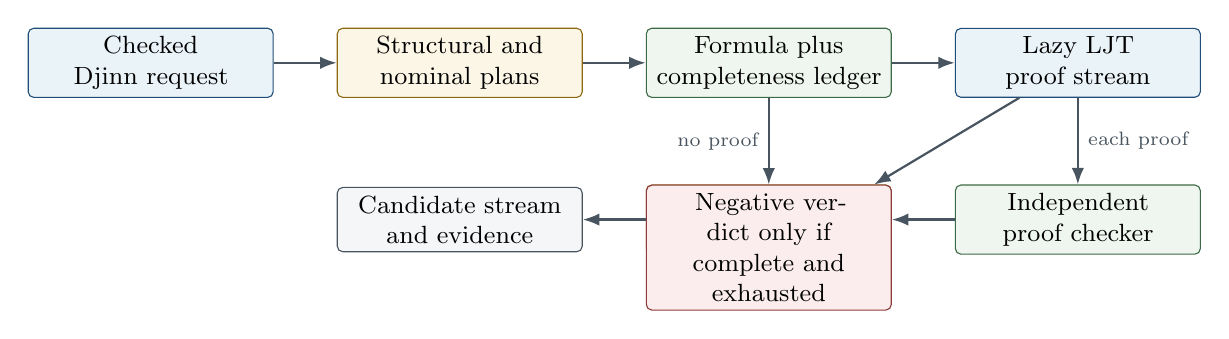
\begin{tikzpicture}[node distance=8mm and 8mm]
  \node[box] (request) {Checked\\Djinn request};
  \node[goldbox,right=of request] (plans) {Structural and\\nominal plans};
  \node[greenbox,right=of plans] (formula) {Formula plus\\completeness ledger};
  \node[box,right=of formula] (ljt) {Lazy LJT\\proof stream};
  \node[greenbox,below=11mm of ljt] (check) {Independent\\proof checker};
  \node[goldbox,left=of check] (lower) {Proof-to-generated\\lowering};
  \node[graybox,left=of lower] (candidate) {Candidate stream\\and evidence};
  \node[redbox,below=11mm of formula] (negative) {Negative verdict only if\\complete and exhausted};

  \draw[flow] (request) -- (plans);
  \draw[flow] (plans) -- (formula);
  \draw[flow] (formula) -- (ljt);
  \draw[flow] (ljt) -- node[right,note]{each proof} (check);
  \draw[flow] (check) -- (lower);
  \draw[flow] (lower) -- (candidate);
  \draw[flow] (formula) -- node[left,note]{no proof} (negative);
  \draw[flow] (ljt) -- (negative);
\end{tikzpicture}}
\caption{Djinn's proof-producing pipeline. The negative edge is guarded by both compiler completeness and search exhaustion.}
\label{fig:djinn-pipeline}
\end{figure}

\section{Core orchestration and instantiation axioms}

\dpath{djinn/src-core/Djinn/Core.hs} orchestrates plan construction, premise selection, LJT execution, proof validation, deduplication, ranking, and evidence. The file is large because it is where independent correctness conditions meet.

The engine can derive several classes of controlled instantiation premise:

\begin{itemize}
  \item closed monotype instantiations available from the query itself;
  \item query-correlated instantiations whose shared variables must receive one coherent assignment;
  \item loaded polymorphic values whose exact schemes are known in the session;
  \item provider-local assignments supplied by an external frontend or compiler integration;
  \item visible type-application evidence retained in the generated term.
\end{itemize}

These are not unconstrained axioms. Each is created from a checked source scheme, exact argument vector, kind proof, and plan-retention check. After the proof checker validates a derivation in the enriched proof environment, the instantiation evidence is rewritten or erased in a controlled lowering step so the generated term refers to actual source values and visible type applications rather than fictional logical constants.

\section{Proof checking and lowering}

Every LJT proof is passed to \dpath{djinn/src-core/Djinn/Internal/ProofCheck.hs}. The checker reconstructs the derivation against the formula and proof environment. Search ordering, cached reachability, and heuristic plan choice are not trusted as proof evidence.

Accepted proofs are converted by \dpath{djinn/src-core/Djinn/Internal/ProofToGenerated.hs}. The lowering pass maps logical introductions and eliminations to lambda, application, tuple, constructor, and case syntax; restores source constructor identities; resolves instantiation witnesses; and produces a shared generated clause. Scope is checked again at the shared AST boundary.

\begin{invariantbox}
Djinn's trusted result is not ``the search code said success.'' It is ``the independent checker accepted this proof term for this translated formula, and the lowering pass produced a scoped generated term.'' The final client may still need to check that translation and rendering preserve the source-language goal.
\end{invariantbox}

\section{Evidence outcomes}

Conceptually, the core can distinguish:

\begin{itemize}
  \item \term{realized}: one or more checked candidates exist;
  \item \term{unrealizable}: exhaustive complete search found no proof;
  \item \term{unrealizable without self-reference}: a diagnostic run proves that only reintroducing the target enables a proof;
  \item \term{undecided}: a budget, incomplete plan family, opaque unsupported structure, or other limitation prevents a verdict.
\end{itemize}

A global candidate cutoff is shared across plans. To know whether the cutoff actually truncated a nonempty tail, the implementation observes one extra proof as a witness. Choice-point budgets are likewise shared across plan execution rather than reset per plan. Otherwise a caller requesting a budget of \(N\) could accidentally receive \(N\) work for every structural plan.

Candidates from different plans are deduplicated after normalization, including structural and eta-equivalent forms where the shared representation can establish equivalence. Optional ranking favors compact terms and can consider unused-binder ratios.

\section{Worked trace: identity}

For \code{forall a. a -> a}, a representative trace is:

\begin{enumerate}
  \item Request preparation validates one leading forall and no class context.
  \item A positive-forall plan opens \code{a} as a fresh rigid proposition symbol.
  \item The compiler emits \(a \to a\).
  \item Right implication introduction extends the antecedent with \(x:a\) and sets goal \(a\).
  \item The atomic goal is discharged from the antecedent, yielding a variable proof.
  \item The proof is wrapped in a lambda, normalized, and checked.
  \item Lowering emits a lambda over one local binder.
  \item The plan family may also consider an opaque interpretation, but deduplication removes equivalent forwarding terms.
\end{enumerate}

The apparent triviality is misleading. The same machinery must retain alpha identity if the forall is nested, avoid opening it at a negative polarity without evidence, and keep the binder rigid in the proof environment.

\section{Worked trace: swapping a product}

For \code{(a,b) -> (b,a)}, the compiler emits a conjunction implication. Search introduces the input, splits it into two components, constructs a conjunction in reverse order, and returns a proof term using tuple split and tuple construction. Lowering chooses a generated pattern/case representation. Later frontends may render it as a tuple-pattern lambda or as an explicit match depending on target-language constraints.

This trace is a useful debugging probe because it crosses both an elimination and an introduction, exercises binder scopes created by a destructuring pattern, and reveals whether normalization preserves constructor descriptions.

\section{Debugging Djinn}

When Djinn unexpectedly returns no term, inspect in this order:

\begin{enumerate}
  \item Was the public query rejected or was a checked request actually constructed?
  \item Which type regions became opaque, and did the compiler mark translation incomplete?
  \item Which structural plans were generated and which exact assignments survived each plan?
  \item Were relevant loaded values or constructors omitted by premise policy?
  \item Did the LJT stream exhaust, hit a choice-point budget, or hit the candidate cutoff?
  \item Did a proof appear but fail \code{ProofCheck}?
  \item Did lowering or generated-scope validation reject it?
  \item Did client-side rendering or final source elaboration reject the neutral candidate?
\end{enumerate}

The distinction between steps 5, 6, and 8 is particularly important. A proof-search defect, a proof-checker rejection, and a downstream source-validation rejection require entirely different fixes.

\begin{sourcebox}
The shortest source trail through a Djinn request is: \dpath{djinn/src-core/Language/Haskell/Djex/Djinn.hs} $\rightarrow$ \dpath{djinn/src-core/Language/Haskell/Djex/Djinn/Internal/Request.hs} $\rightarrow$ \dpath{djinn/src-core/Djinn/Core.hs} $\rightarrow$ \dpath{djinn/src-core/Djinn/Internal/TypeFormula.hs} $\rightarrow$ \dpath{djinn/src-core/Djinn/Internal/LJT.hs} $\rightarrow$ \dpath{djinn/src-core/Djinn/Internal/ProofCheck.hs} $\rightarrow$ \dpath{djinn/src-core/Djinn/Internal/ProofToGenerated.hs}.
\end{sourcebox}

\chapter{Exference: typed-hole search, ranking, and reconstruction}\label{ch:exference}

\section{What Exference promises}

Exference is the heuristic and ranking-oriented backend. It searches a state space of partially constructed typed expressions. Nodes contain typed holes, lexical scopes, rigid and flexible type variables, class obligations, globals, exact provider evidence, constructor/deconstructor knowledge, usage counts, freshness supplies, and a priority score. The scheduler expands the most promising node, bounds the queue and depth, and emits solved expressions. An independent checker reconstructs each candidate before it crosses the adapter boundary.

Exference is often better than Djinn when a useful term should call a library value, when several plausible terms need ranking, or when rank-N elimination and explicit type applications are involved. Its negative result is intentionally weaker: it does not claim that queue exhaustion proves uninhabitability.

The adapter starts at \dpath{exference/src-core/Language/Haskell/Djex/Exference.hs}; the central scheduler is \dpath{exference/src-core/Language/Haskell/Exference/Core/Internal/Exference.hs}; node data and construction are in \dpath{exference/src-core/Language/Haskell/Exference/Core/Internal/ExferenceNode.hs} and \dpath{exference/src-core/Language/Haskell/Exference/Core/Internal/ExferenceNodeBuilder.hs}.

\section{Checked environment and request}

The adapter builds an opaque Exference session from the shared environment. It projects declarations, class information, constructor/deconstructor bindings, ratings, visibility, and prepared schemes into Exference-specific authorities. Projection can omit unsupported declarations, but omissions are returned as diagnostics rather than silently changing the query.

A checked Exference query seals together:

\begin{itemize}
  \item the exact prepared environment;
  \item the normalized goal and explicit contexts;
  \item global and local source-name mappings;
  \item provider candidates and exact assignments;
  \item a rigid-instantiation plan;
  \item search options and penalty overrides.
\end{itemize}

Assignment validation checks exact provider scheme identity, argument count, absence or treatment of contexts, kinds, closure, finite widths, and duplicates. A textual name match is insufficient.

\section{Types and unification}\label{sec:exference-unify}

The core reuses the shared neutral type through compatibility patterns. \dpath{exference/src-core/Language/Haskell/Exference/Core/Types.hs} defines Exference-facing views, substitutions, polytype helpers, and scope-sensitive operations. The actual unifier is \dpath{exference/src-core/Language/Haskell/Exference/Core/Unify.hs}.

\subsection{Disjoint and shared namespaces}

Exference needs several unification modes. Two schemes may use the same integer identifiers but mean different variables; a local expression and a global scheme may share a rigid scope; a right-hand pattern may contain the only variables permitted to bind. The API therefore distinguishes disjoint, shared, and one-sided unification rather than relying on caller folklore.

Internally, variables are tagged with their origin before unification. This prevents accidental capture or identification merely because two integer supplies both started at zero.

\subsection{Higher-kinded heads}

The unifier observes a constructor-application form. Functions and tuples can be lowered to canonical heads for this purpose, so a flexible head variable can bind to a type constructor of the right kind. Kind checking is not deferred until rendering: a substitution that solves the first-order shape but violates kind arity is rejected.

\subsection{Opaque polytypes}

Nested polytypes become tagged opaque atoms. They can unify as complete values when their alpha-normal keys and substitutions agree, but the unifier cannot decompose a forall under an application as if it were a monotype. Occurs checks still inspect the atom's free variables. Substitution into the atom is capture-avoiding.

\begin{invariantbox}
A nested forall is simultaneously opaque to structural decomposition and transparent to lexical hygiene. ``Opaque'' never means ``free-variable blind.''
\end{invariantbox}

\section{Classes and residual constraints}

Exference builds a static class environment from validated class and instance declarations. It checks duplicate or overlapping instance heads according to the supported policy, class arity, superclass cycles, and recursively expanding prerequisites. Search may carry scoped givens and unresolved obligations. A solved expression is only a candidate after constraint closure determines which residual constraints are valid and whether they escape the permitted scope.

The expression checker later recomputes residual constraints and compares them with the candidate's claimed set. Search cannot simply attach a convenient list.

\section{The search node}\label{sec:exference-node}

A node is a complete snapshot of one partial program. Important fields include:

\begin{itemize}
  \item pending typed holes and the already selected next goal;
  \item a scope forest describing lexical parentage;
  \item local givens and scoped class constraints;
  \item flexible substitutions and rigid scopes;
  \item global bindings with exact schemes and source identities;
  \item visible type-application candidates;
  \item provider candidate and assignment maps;
  \item constructor and deconstructor bindings;
  \item per-binding usage counts and donation guards;
  \item the current annotated generated expression;
  \item fresh supplies for term variables, type variables, scopes, and holes;
  \item accumulated depth, last selected binding, and score inputs.
\end{itemize}

The apparent duplication is deliberate. Search branches must be clonable and self-describing. A node should not depend on mutable ambient state whose meaning changes after it is enqueued.

\subsection{Typed goals}

A pending goal records a hole identifier, expected type, lexical scope, forall-introduction mode, tuple policy, and local givens. Forall goals can be in phases such as opening an existing leading prefix, trying an introduction, or continuing a previously selected introduction. Tuple goals can choose a shallow structural lane or a whole-tree shortcut. These modes prevent one generic expansion rule from repeatedly rediscovering the same administrative choices.

\subsection{Freshness and identifier exhaustion}

Node construction uses explicit finite supplies. If a fresh identifier cannot be allocated within the supported space, the branch records identifier exhaustion and terminates cleanly. Wraparound is never allowed to produce aliasing between an old binder and a new hole.

\section{The scheduler loop}\label{sec:exference-scheduler}

The scheduler maintains a maximum-priority queue of nodes. A scheduled node already has its next goal selected, so the queue ordering is over actionable states rather than states that must perform another non-deterministic pop after dequeue.

One iteration conceptually does the following:

\begin{lstlisting}[language=Haskellish]
step state =
  case popBest state.queue of
    Nothing   -> finishWithExactPruningEvidence state
    Just node ->
      let children = expandSelectedGoal node
          (tooDeep, admissible) = partitionDepth children
          (solved, future)      = partitionSolved admissible
          checked              = checkSolved solved
          scored               = score future
          queue'               = mergeWithCapacity scored state.queue
      in emit checked (updateCounters queue' tooDeep)
\end{lstlisting}

Again, this is explanatory pseudocode. The implementation is careful about laziness, exact prune counts, and continuation state.

\begin{figure}[htbp]
\centering
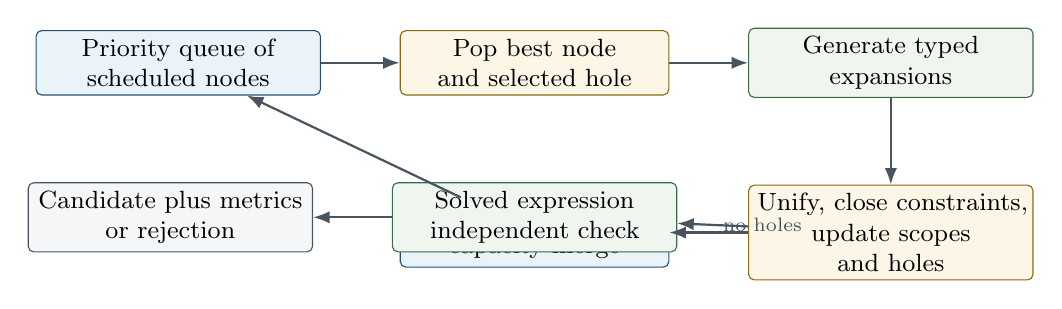
\begin{tikzpicture}[node distance=8mm and 10mm]
  \node[box,text width=34mm] (queue) {Priority queue of\\scheduled nodes};
  \node[goldbox,right=of queue,text width=32mm] (pop) {Pop best node\\and selected hole};
  \node[greenbox,right=of pop,text width=34mm] (expand) {Generate typed\\expansions};
  \node[goldbox,below=11mm of expand,text width=34mm] (unify) {Unify, close constraints,\\update scopes and holes};
  \node[box,left=of unify,text width=32mm] (score) {Score, depth-filter,\\capacity-merge};
  \node[greenbox,below=11mm of pop,text width=34mm] (solved) {Solved expression\\independent check};
  \node[graybox,left=of solved,text width=34mm] (candidate) {Candidate plus metrics\\or rejection};

  \draw[flow] (queue) -- (pop);
  \draw[flow] (pop) -- (expand);
  \draw[flow] (expand) -- (unify);
  \draw[flow] (unify) -- (score);
  \draw[flow] (score) -- (queue);
  \draw[flow] (unify) -- node[right,note]{no holes} (solved);
  \draw[flow] (solved) -- (candidate);
\end{tikzpicture}
\caption{The Exference search loop. Queue pruning and depth pruning are measured, not inferred after the fact. Solved nodes bypass the queue and enter a separate checking path.}
\label{fig:exference-loop}
\end{figure}

\subsection{Queue capacity and exact pruning}

A bounded queue keeps the search operational in large libraries. The merge routine must retain the best nodes under the ordering while reporting exactly how many were discarded. It cannot append two queues, truncate, and then guess which source lost nodes. Those exact counts become \code{QueueLimitPruned} and contribute to progress.

Depth pruning is recorded separately. A final empty queue after any pruning means ``no remaining node under this policy,'' not ``the type is impossible.''

\subsection{Expansion families}

Depending on the goal, expansion can:

\begin{itemize}
  \item introduce a lambda binder;
  \item open or preserve a forall;
  \item choose a local or global binding and create argument holes;
  \item insert visible type applications from exact evidence;
  \item construct a tuple or data constructor;
  \item eliminate a tuple or data value through a case;
  \item use a provider with an occurrence-local assignment;
  \item introduce a let or reuse a previously built value;
  \item carry or discharge class obligations.
\end{itemize}

Every expansion updates the expression and the type state together. A term edge without the corresponding substitution, scope, and hole changes is not a valid child node.

\section{Scoring and usage}

The score combines structural complexity, configured binding ratings, type complexity, depth, class burden, provider penalties, usage policy, and other heuristic features. Source ratings are inputs, not proof evidence. A client can supply relevance-biased overrides for providers discovered from its source environment.

Usage counts serve several purposes. They can prefer candidates that use requested arguments, reject candidates with unused binders under a strict lane, and provide backend metrics. The strict and relaxed policies are often run as separate lanes rather than one score penalty, because ``unused forbidden'' is a semantic filter while ``unused discouraged'' is a heuristic.

\section{Expression representation}

\dpath{exference/src-core/Language/Haskell/Exference/Core/Expression.hs} wraps the shared generated syntax with annotated locals carrying internal identifiers and optional type information. Compatibility pattern synonyms preserve older Exference-facing constructors while the storage representation converges on the shared AST.

The conversion boundary erases search-only annotations only after scope and typing checks. This is another example of keeping a richer internal proof object until the last responsible moment.

\section{The independent expression checker}\label{sec:exference-checker}

\dpath{exference/src-core/Language/Haskell/Exference/Core/Internal/ExpressionCheck.hs} is the key trust boundary; the historical module \dpath{exference/src-core/Language/Haskell/Exference/Core/ExpressionCheck.hs} is now a small re-export shim that preserves the original surface over that internal implementation. The checker does not accept the search node's accumulated typing story as a derivation. It reconstructs the expression bidirectionally against an opaque prepared checker context.

The checker validates:

\begin{itemize}
  \item generated-tree well-formedness and absence of holes;
  \item local binder scope and global source identity;
  \item applications, lambdas, tuples, constructors, lets, and cases;
  \item nested forall introduction and visible type application;
  \item rigid-scope provenance and absence of escaping rigids;
  \item constructor/deconstructor schemes;
  \item class givens and residual obligations;
  \item exact equality between reconstructed and claimed residual constraints.
\end{itemize}

It reuses the pure unification kernel because duplicating unification would create two semantics. It does not reuse the search scheduler, queue ordering, score, or node-local assumption that a hole had a certain type. Search contributes only irreducible provenance that cannot be recovered from the erased expression, such as the origin of certain nested rigid instantiations.

The simplified candidate is checked first. If simplification changed a representation in a way the checker rejects, the raw expression may be checked as a fallback. A candidate that fails both is dropped with diagnostics; it is not exposed as ``probably typed.''

\begin{designbox}
The independent checker turns Exference from a heuristic term generator into a checked heuristic term generator. The search can be aggressively optimized or reordered without making every optimization part of the trusted typing argument.
\end{designbox}

\section{Adapter output and defensive rendering}

The stable adapter converts checked internal candidates to shared candidates and attaches metrics such as steps, penalty, final queue size, binding usage, and exact pruning totals. Residual constraints and generated scope are validated again.

Diagnostic hints can originate in user or source text and may be cyclic or infinite in a lazy language. Pure rendering observes a bounded prefix and catches synchronous exceptions while preserving asynchronous exceptions. A bad hint must not take down an otherwise valid search result.

\section{Worked trace: applying a provider}

Consider a goal corresponding to \code{(a -> b) -> F a -> F b} with a provider \code{mapF : forall x y. (x -> y) -> F x -> F y}.

\begin{enumerate}
  \item The root forall prefix creates rigid type variables \code{a} and \code{b}.
  \item Arrow introduction puts \code{f : a -> b} and \code{xs : F a} in scope.
  \item The result hole expects \code{F b}.
  \item Selecting \code{mapF} instantiates its two quantified variables. Exact provider evidence correlates \code{x=a} and \code{y=b} at this occurrence.
  \item The instantiated result unifies with \code{F b}; two argument holes are created for \code{a -> b} and \code{F a}.
  \item Local selection fills them with \code{f} and \code{xs}.
  \item The solved expression contains a global provider occurrence plus visible type applications when required by the source scheme.
  \item The independent checker reconstructs the scheme instantiation and local applications.
\end{enumerate}

This trace exercises the features for which Exference's rich state is justified: occurrence-local assignments, explicit instantiation, global/local scope, and ranking of a library-oriented term.

\section{Why Exference does not refute}

Even a completely empty final queue may be the result of:

\begin{itemize}
  \item a finite step limit;
  \item queue-capacity pruning;
  \item depth pruning;
  \item a finite identifier supply;
  \item disabled expansion families;
  \item ranking that starved a productive region before the limit;
  \item an intentionally incomplete provider or declaration projection;
  \item candidate policies such as forbidding unused binders.
\end{itemize}

The adapter reports these conditions precisely. It never upgrades them to a logical proof. A combined client must preserve this asymmetry: an Exference miss can neither cancel nor create a Djinn refutation.

\section{Djinn and Exference compared}

\begin{longtable}{@{}L{0.19\textwidth}L{0.36\textwidth}L{0.36\textwidth}@{}}
\toprule
\textbf{Dimension} & \textbf{Djinn} & \textbf{Exference} \\
\midrule
\endhead
Internal object & Formula, sequent state, proof term & Typed expression with holes, scopes, substitutions, queue state \\
Primary strength & Structural/proof-theoretic synthesis and conditional negative evidence & Ranked library/provider-oriented synthesis and richer elimination/instantiation \\
Ordering & Calculus strategy and plan family & Priority score with queue/depth limits \\
Independent validation & Proof checker & Bidirectional expression checker \\
Rank-N treatment & Opaque-by-default formula plans plus checked instantiation axioms & Opaque polytypes, rigid scopes, visible type applications, occurrence-local assignment \\
Negative result & Possible when translation and search are complete & Never promoted to proof of uninhabitability \\
Candidate ranking & Optional, comparatively light & Core design feature with ratings and usage metrics \\
Typical failure question & ``Was translation/search complete?'' & ``Which policy, score, or bound removed the productive node?'' \\
\bottomrule
\end{longtable}

\begin{sourcebox}
The shortest Exference source trail is: \dpath{exference/src-core/Language/Haskell/Djex/Exference.hs} $\rightarrow$ \dpath{exference/src-core/Language/Haskell/Djex/Exference/Internal/Request.hs} $\rightarrow$ \dpath{exference/src-core/Language/Haskell/Exference/Core/Internal/ExferenceNodeBuilder.hs} $\rightarrow$ \dpath{exference/src-core/Language/Haskell/Exference/Core/Internal/Exference.hs} $\rightarrow$ \dpath{exference/src-core/Language/Haskell/Exference/Core/Unify.hs} $\rightarrow$ \dpath{exference/src-core/Language/Haskell/Exference/Core/Internal/ExpressionCheck.hs} (reached historically through the \code{Core.ExpressionCheck} re-export shim).
\end{sourcebox}

\chapter{The unified facade, source frontends, and REPL}\label{ch:djex-facade}

\section{A capability-aware facade}

\dpath{src/Language/Haskell/Djex.hs} is the preferred programmatic entry surface. It defines the backend selection, common session/query operations, and an explicit capability vocabulary. Capabilities include deciding inhabitation, heuristic search, prenex polymorphism, rank-N introduction and elimination, opaque rank-N transport, impredicative support, ranked candidates, and type-class constraints.

The capability matrix is executable documentation. A client can choose Djinn when a complete structural negative result matters, Exference when ranking or elimination matters, or both when it can merge candidates while respecting asymmetric evidence.

The public surface is now larger than backend selection, sessions, and capabilities. Beyond the original shared vocabulary, the facade re-exports sixteen further modules: \code{Fingerprint}, \code{Observability}, \code{TypeInstantiation}, \code{TypedCandidate}, \code{TypedGenerated} and \code{TypedGenerated.Fingerprint}, and ten \code{Semantic.*} modules covering the Length domain, its SMT-LIB encoding and live Z3 boundary, and the generic behavioral-problem envelope (Section~\ref{sec:semantic-stratum}).

\begin{invariantbox}
A facade may normalize calling conventions, but it may not normalize away semantic differences. ``No candidates'' has backend-specific meaning and remains so after dispatch.
\end{invariantbox}

\section{Source conversion}

\dpath{src/Language/Haskell/Djex/HaskellSrc.hs} and the historical frontend conversion modules parse Haskell source declarations into the shared environment vocabulary and render generated terms back to Haskell-like source. The conversion boundary handles qualification, operator names, source locations, fixities where supported, class declarations, and the mismatch between source syntax and neutral AST structure.

The historical Exference frontend under \filepath{exference/src-frontend/Language/Haskell/Exference} includes environment parsing, declaration extraction, source-type conversion, class-environment construction, expression rendering, and CLI support. The historical Djinn frontend under \filepath{djinn/src-frontend} retains its original command vocabulary and help surface.

These frontends are useful compatibility layers, but new semantic changes should enter through shared authorities and checked adapters. Adding a type feature only to a source parser creates a value neither backend has promised to understand.

\section{Packages, workspaces, and dependency order}

\dpath{src/Language/Haskell/Djex/Package.hs} and \dpath{src/Language/Haskell/Djex/REPL/Workspace.hs} manage packages and workspaces. A workspace is not merely a list of files. It must resolve module identities, dependencies, declaration order, loaded environments, and command-line tool interaction. \dpath{src/Language/Haskell/Djex/Internal/DependencyGraph.hs} supplies dependency ordering and cycle handling.

Package discovery can invoke Cabal-facing tooling. Test support includes a fake Cabal executable (\code{djex-fake-cabal}) so CLI behavior can be tested without making unit tests depend on a user's machine configuration, and a fake Z3 executable (\code{djex-fake-z3}, \dpath{test-support/fake-z3/Main.hs}) that stands in for a live solver worker under closed fault modes and keeps the empty-child-environment and fresh-working-directory launch policies observable in tests.

\section{The unified REPL}

The large \dpath{src/Language/Haskell/Djex/REPL.hs} coordinates the interactive session. Focused submodules divide concerns:

\begin{longtable}{@{}L{0.31\textwidth}L{0.61\textwidth}@{}}
\toprule
\textbf{Module} & \textbf{Responsibility} \\
\midrule
\endhead
\dpath{src/Language/Haskell/Djex/REPL/Command.hs} & Command grammar, abbreviations, arguments, and command-level diagnostics. \\
\dpath{src/Language/Haskell/Djex/REPL/Driver.hs} & Input loop, prompt, multiline behavior, output and exception boundary. \\
\dpath{src/Language/Haskell/Djex/REPL/Scope.hs} & Visible declarations, qualification, ambiguity, namespace resolution, and import/export effects. \\
\dpath{src/Language/Haskell/Djex/REPL/Type.hs} & Type parsing, normalization, checking, and user-facing type operations. \\
\dpath{src/Language/Haskell/Djex/REPL/Kind.hs} & Kind queries and diagnostics. \\
\dpath{src/Language/Haskell/Djex/REPL/Eval.hs} & Evaluation-oriented commands and source execution boundaries. \\
\dpath{src/Language/Haskell/Djex/REPL/DjinnScope.hs} & Projection of the unified visible scope into Djinn-specific premise policy. \\
\dpath{src/Language/Haskell/Djex/REPL/Workspace.hs} & Workspace loading, module graph, package context, and reload behavior. \\
\bottomrule
\end{longtable}

The top-level REPL maintains both source-facing state and backend sessions. A declaration update must rebuild or increment every dependent authority in a defined order. The REPL should never retain an Exference session built from environment version \(n\) while rendering against source scope version \(n+1\).

\section{Commands and the CLI}

\dpath{src/Language/Haskell/Djex/Command.hs} defines shared command structures, while \dpath{src/Language/Haskell/Djex/CLI.hs} handles process arguments, modes, files, and startup behavior. \dpath{src/Language/Haskell/Djex/Text.hs} centralizes bounded text helpers and presentation details.

The package builds five executables. The three installable ones---\code{djex}, \code{djinn}, and \code{exference}---are intentionally thin at their \filepath{app/Main.hs} entry points. Substantive process behavior lives in library modules, which is why CLI tests can call command logic without forking for every assertion while still retaining end-to-end executable tests. The two private test fixtures are different in kind: \code{djex-fake-cabal} is a small Cabal stand-in, while \code{djex-fake-z3} (\dpath{test-support/fake-z3/Main.hs}, 538 lines) is a deliberately substantial closed-fault-mode Z3 stand-in whose behavior is selected only by its copied executable name, never by a sibling file, inherited environment variable, or working-directory entry.

\section{Extension discipline}

A safe feature generally lands in this order:

\begin{enumerate}
  \item add or refine a shared authority and its pure tests;
  \item update environment/inventory validation and kind inference;
  \item teach Djinn's adapter/compiler only what it can soundly translate;
  \item teach Exference's adapter/unifier/search/checker only what it can reconstruct;
  \item update the generated AST if a genuinely new term form is required;
  \item update source frontends and renderers;
  \item expose a capability bit or diagnostic when support is asymmetric;
  \item add facade, REPL, CLI, and integration tests.
\end{enumerate}

Starting at the REPL and working downward usually creates a period in which text syntax exists without a validated semantic path.

\chapter{Djex tests, benchmarks, and diagnostic workflow}\label{ch:djex-tests}

\section{Concentric test layers}

The repository's test organization mirrors its trust boundaries. The package now declares sixteen test suites; the table lists the boundary each layer protects.

\begin{longtable}{@{}L{0.28\textwidth}L{0.64\textwidth}@{}}
\toprule
\textbf{Suite} & \textbf{What it protects} \\
\midrule
\endhead
\dpath{synthesis/test/Spec.hs} & Shared names, types, substitution, alpha equivalence, environments, kind inference, queries, generated syntax, inventories, finite-width guards, and diagnostics. The suite also compiles \code{ClassResolutionSpec} and seven SMT-LIB spec modules with their \filepath{synthesis/internal} subjects as home modules, so package-private code is tested without becoming public. \\
\dpath{synthesis/test-length/Spec.hs} & The Length/SMT-LIB/Z3 semantic stack, including the live-worker specs. At roughly 12{,}500 lines this is the largest file in the repository. \\
\dpath{synthesis/test-certificate/Spec.hs} & Type-application certificate plans and typed-candidate association. \\
\dpath{synthesis/test-fingerprint/Spec.hs} & Canonical fingerprint encoding and behavioral-problem identity. \\
\dpath{synthesis/test-term-graph-fingerprint/Spec.hs} & Typed term-graph fingerprint identity at the public entrance. \\
\dpath{djinn/test-unit/Spec.hs} & Formula translation, LJT rules, normalization, instantiation plans, proof checking, lowering, evidence, budgets, and regressions. \\
\dpath{djinn/test-property/PropertySpec.hs} & Property-level relationships such as checker acceptance, normalization, and generated-term invariants over broad inputs. \\
\dpath{exference/test-unit/Spec.hs} & Unification, rigid scopes, class closure, node expansion, scoring, provider assignments, expression checking, pruning, and regressions. \\
\dpath{exference/test-engine/EngineSpec.hs} & Black-box engine behavior with checked environments and bounded search. \\
\dpath{test-api/AbstractionBoundary.hs} & Compile-time enforcement that internal constructors and modules do not leak through the supported public API. \\
\dpath{test-api/FacadeSpec.hs} & Backend dispatch, capability reporting, common query behavior, and facade diagnostics. \\
\dpath{test-integration/Spec.hs} & Cross-layer behavior: source declarations through sessions and engines to rendered candidates and evidence. \\
\dpath{test-cli/Spec.hs} & Unified command-line and REPL protocol, formatting, files, workspaces, package discovery, and failure behavior. \\
Historical CLI/API suites & Compatibility of the retained \code{djinn} and \code{exference} entry surfaces. \\
\bottomrule
\end{longtable}

The abstraction-boundary tests deserve special attention. In Haskell, a module export list is part of the correctness story. If a constructor becomes public accidentally, downstream code can fabricate a value that bypasses every runtime test. Compile-time negative tests guard that boundary.

\section{Benchmarks}

Both historical engines have benchmark corpora. A useful benchmark change should record more than wall-clock time. For Djinn, track proof-plan counts, choice points, proof prefix latency, and deduplication. For Exference, track steps, peak/final queue size, exact queue/depth pruning, candidate rank, and checker rejection. A speedup that changes the first accepted candidate or turns finished search into truncation is a semantic change and should be reviewed as such.

\section{A practical failure funnel}\label{sec:djex-failure-funnel}

When a top-level test says ``expected candidate, got none,'' localize the loss:

\begin{enumerate}
  \item \term{Source conversion}: did the declaration or goal parse to the intended shared type?
  \item \term{Environment}: did validation retain the declaration and indexes?
  \item \term{Projection}: did the selected backend session include the value, constructor, class, or instance?
  \item \term{Request}: did exact contexts and provider assignments survive checked preparation?
  \item \term{Search}: did the backend generate a proof/node, or did a bound/prune intervene?
  \item \term{Internal checker}: did proof or expression reconstruction reject it?
  \item \term{Shared AST}: did scope, simplification, or candidate conversion reject it?
  \item \term{Frontend}: did qualification or source rendering reject or duplicate it?
\end{enumerate}

Instrumenting all eight at once produces noise. Add a probe at the earliest boundary whose output is wrong.

\section{Negative-evidence tests}

The most valuable negative tests are not examples of impossible types; they are examples where a tempting implementation would falsely claim impossibility. Include cases with:

\begin{itemize}
  \item a search budget reached just before a proof;
  \item an omitted rank-N structural plan;
  \item an opaque nominal type that must be forwarded;
  \item a recursive type whose one-layer exposure is incomplete;
  \item a provider assignment that a plan fails to retain exactly;
  \item target self-reference excluded from the safe environment;
  \item Exference queue/depth pruning followed by an empty queue.
\end{itemize}

These tests protect the distinction between ``no proof exists'' and ``this implementation did not find one.''

\begin{summarybox}
Djex's test suite is best read as a map of trusted boundaries. Pure shared tests establish authorities; backend tests establish search and checking; API tests establish encapsulation; integration and CLI tests establish that the boundaries compose.
\end{summarybox}


\part{Traces, diagnostics, and maintainer guide}

\chapter{Concrete Djex traces}\label{ch:djex-traces}

These traces are deliberately backend-neutral at the entrance. They show where Djinn and Exference diverge and where they rejoin the shared result boundary.

\section{Trace A: polymorphic identity}

Take
\[
  \forall a.\;a \to a.
\]
The shared representation is one leading \code{ForallType} and one \code{FunctionType}. Djinn implicitizes the prefix, compiles the body to \(A \to A\), introduces the antecedent, and closes by identity. The proof checker validates a single lambda proof; lowering produces a clause whose expression is \code{Lambda [Bind x] (Local x)}.

Exference opens the leading forall with a rigid instantiation, introduces one local value, and fills the result hole from that local. The strict unused-binder policy accepts the result because the argument is used once. The independent checker reconstructs the same rigid type and validates the generated scope.

This is the smallest useful boundary test. If it fails, check binder implicitization, rigid/flexible tagging, scope insertion, generated local identity, and result-envelope construction before investigating ranking or complex declarations.

\section{Trace B: product swap}

For
\[
  (a,b) \to (b,a),
\]
shared canonicalization stores the saturated tuple structurally. Djinn compiles the input product as a conjunction and the output as the reverse conjunction. Its proof uses conjunction-left followed by conjunction-right. Proof lowering emits either a tuple pattern or an explicit split followed by tuple construction, then shared simplification removes redundant structure.

Exference selects tuple introduction for the result, creating two holes. It deconstructs the input in a child scope and fills the holes in reverse order. The scope forest prevents a field binder from escaping its branch. The independent checker validates constructor/deconstructor arity and both component types.

A plausible-looking but wrong result usually points to one of four places: tuple constructor canonicalization, deconstructor parameter order, pattern binding-site traversal, or generated simplification.

\section{Trace C: sum elimination}

For the Haskell-like type
\[
  (a \to c) \to (b \to c) \to \mathrm{Either}\;a\;b \to c,
\]
Djinn represents \code{Either} as a labeled disjunction. Disjunction-left creates one proof branch for each constructor payload; each branch applies the corresponding function. Constructor descriptors retain name and arity so proof checking and generated case lowering agree.

Exference schedules a deconstruction of the sum input, creates branch-local scopes, and searches a result hole in each branch. The \code{a} payload cannot appear in the \code{b} branch because the scope tree, goal scope ID, and independent expression checker all enforce locality.

When adding a new multi-constructor datatype path, test both introduction and elimination. A constructor-only test does not exercise branch scopes, and an elimination-only test does not prove that generated constructor metadata is canonical.

\section{Trace D: an exact polymorphic provider}\label{sec:djex-provider-trace}

Suppose a session contains a value morally equivalent to
\[
  \mathit{map} : \forall f\,a\,b.\;(a \to b) \to f\,a \to f\,b,
\]
and an external compiler frontend has established the exact assignment \((\mathrm{List}, A, B)\) for one occurrence.

The frontend supplies one kinded provider assignment. The adapter checks the provider's exact retained scheme, the three binder kinds, the vector arity, closure of each argument, synonym meaning, and final specialization kind. The assignment remains attached to that provider rather than entering a global pool.

Djinn may turn the specialization into a checked synthetic premise and visible-application rewrite. Proof search can use the premise, proof checking sees the synthetic symbol, and lowering rewrites the occurrence back through the exact provider with its visible type arguments. Exference stores the correlated vector in the search node; selecting the provider consumes the complete assignment directly and preserves the visible application in the generated expression.

A bug in this path often appears only when two providers have alpha-equivalent schemes or when two assignments share individual arguments but differ as vectors. Regression tests should therefore include multiple providers, repeated type variables, higher-kinded arguments, and reordered near misses.

\section{Trace E: rank-N forwarding versus elimination}\label{sec:djex-rankn-trace}

Rank-N support has two qualitatively different cases.

\subsection{Opaque forwarding}

For
\[
  (\forall a.\;a \to a) \to (\forall a.\;a \to a),
\]
the nested forall can remain one alpha-aware \code{TypeAtom}. Djinn treats it as an opaque proposition and proves identity without inspecting the body. Exference's unifier treats the quantified value as an indivisible atom while still substituting its free variables capture-safely. Both engines can therefore forward a polymorphic value exactly.

\subsection{Elimination}

For
\[
  (\forall a.\;a \to a) \to \mathrm{Int} \to \mathrm{Int},
\]
the local polymorphic value must be instantiated. Exference can open the local scheme at the use site under a rigid-scope plan and emit a visible type application. Djinn requires one of its bounded instantiation mechanisms: a query-derived closed candidate, a correlated assignment, or another checked axiom family. The generated AST retains the visible type argument; no renderer is asked to recover it from a proof-variable spelling.

The distinction matters when changing opacity. Opening every forall would lose exact forwarding and make negative evidence depend on an arbitrarily aggressive translation. Keeping every forall opaque would lose useful introduction and elimination. The code instead records a bounded family of coherent plans.

\section{Trace F: recursive datatypes}

The type \code{List a -> List a} should be solved by forwarding without unfolding recursion. Djinn's exact opaque plan preserves that path even when a positive recursive projection exposes one constructor layer in another plan. Exference can likewise select the input directly without deconstruction.

A goal that constructs one visible layer, such as \code{a -> List a} in an environment with an admitted one-layer recursive projection, exercises the opposite direction. Djinn may use bounded positive recursive introduction; Exference may choose the constructor and create field holes. Neither engine is licensed to invent unbounded general recursion merely because a source datatype is recursive.

Negative evidence must be weakened whenever recursive unfolding or atomization makes the translation incomplete. A returned proof remains valid for its plan; absence of a proof does not become a refutation of the richer source type.

\section{Trace G: a sound candidate-free result}

Consider \(a \to b\) with no relation between the atoms and no external premises. Djinn compiles a complete first-order formula. In unbudgeted mode, LJT exhausts the proof space. If the target-named assumption was excluded and diagnostic reintroduction also finds no proof, the adapter may return \code{ProvedUninhabitable} with \code{Finished} progress.

The same Exference query may run until its queue is empty and return no candidates. Its result remains \code{NoEvidence}: the algorithm explored its configured search calculus, but the adapter makes no theorem-level claim from that fact.

This paired test is the canonical guard against collapsing evidence into completion. A facade or selector that reports both outcomes identically has erased the most important semantic distinction in Djex.

\chapter{Debugging and operational reasoning}\label{ch:djex-debugging}

\section{Classify the boundary first}

Before instrumenting an engine loop, identify the last authority that accepted the request.

\begin{longtable}{@{}L{0.28\textwidth}L{0.31\textwidth}L{0.33\textwidth}@{}}
\toprule
\textbf{Symptom} & \textbf{Likely boundary} & \textbf{First files to inspect} \\
\midrule
\endhead
Invalid or surprising name/type diagnostic & Shared vocabulary or request preflight & \dpath{synthesis/src/Language/Haskell/Synthesis/Name.hs}, \dpath{synthesis/src/Language/Haskell/Synthesis/Type.hs}, backend request module. \\
Declaration accepted but lookup/projection wrong & Environment or inventory sealing & \dpath{synthesis/src/Language/Haskell/Synthesis/Environment.hs}, \dpath{synthesis/src/Language/Haskell/Synthesis/Inventory.hs}. \\
Djinn misses an obvious theorem & Formula translation, premise plan, or LJT ordering & \dpath{djinn/src-core/Djinn/Internal/TypeFormula.hs}, \dpath{djinn/src-core/Djinn/Core.hs}, \dpath{djinn/src-core/Djinn/Internal/LJT.hs}. \\
Exference misses an obvious short term & Goal expansion, unification, queue rating, or pruning & \dpath{exference/src-core/Language/Haskell/Exference/Core/Internal/Exference.hs}, \dpath{exference/src-core/Language/Haskell/Exference/Core/Unify.hs}. \\
Backend finds a result but canonical output is empty & Independent checker or generated projection & Djinn proof checker/lowering or Exference expression checker/candidate projection. \\
Candidate renders incorrectly & Generated scope, syntax, qualification, or hint allocation & \dpath{synthesis/src/Language/Haskell/Synthesis/Generated.hs}, \dpath{synthesis/src/Language/Haskell/Synthesis/Candidate.hs}. \\
Wrong negative verdict & Formula completeness, budget propagation, evidence merge & Djinn plan orchestration and \dpath{synthesis/src/Language/Haskell/Synthesis/Query.hs}. \\
\bottomrule
\end{longtable}

\section{Request or session rejection}

Preserve the exact failure order while reducing the case. Record:

\begin{itemize}
  \item the sealed environment's declaration order;
  \item the exact neutral goal and explicit contexts before synonym expansion;
  \item backend options;
  \item source provenance, if any;
  \item provider evidence and its outer/inner observed widths;
  \item whether the failure occurs during request construction, session elaboration, or backend lowering.
\end{itemize}

Do not ``simplify'' a cyclic or lazy compatibility value by forcing it in a debugger. The width preflight is often the behavior under test. Reproduce through the same public constructor so the same sentinel observation and diagnostic precedence are exercised.

\section{Djinn produces no candidate}

Walk the pipeline in this order:

\begin{enumerate}
  \item inspect the elaborated shared goal and contexts;
  \item compare the primary, exact opaque, and complementary formula plans;
  \item inspect active premises separately from target-named diagnostic premises;
  \item check whether provider/instantiation axioms were built and whether their evidence was erased only after proof checking;
  \item run the exact formula through \code{proveWithModeChecked};
  \item check whether the proof stream was cut by budget or candidate limit;
  \item inspect proof-check failure before proof-to-generated lowering;
  \item inspect cross-plan deduplication and candidate ranking last.
\end{enumerate}

If an incomplete plan has no proof, the correct outcome is usually undecided, not uninhabitable. If a complete plan has a proof that disappears later, the defect is almost certainly in proof environment restoration, evidence rewriting, proof lowering, generated validation, or deduplication rather than in LJT.

\section{Exference produces no candidate}

Capture the first few queue transitions rather than dumping every node. For each step, record:

\begin{itemize}
  \item popped priority, current goal, scope ID, and rigid mode;
  \item selected binding or constructor;
  \item resulting substitutions and scoped constraints;
  \item generated branches and any identifier-space exhaustion;
  \item depth and queue pruning counts;
  \item whether a solved node was discarded for unused binders, residual constraints, escaping rigids, simplification failure, or independent checking.
\end{itemize}

An empty final queue is ambiguous operationally. Check \code{SearchBatch} progress and pruning reasons before concluding that the search genuinely exhausted all retained work. A useful debugging experiment is to remove queue/depth bounds while keeping the same step limit; if a candidate appears, the issue is ranking/pruning rather than typing.

\section{Independent checker rejection}

A checker failure is valuable: it proves the search and reconstruction semantics diverged. Preserve both representations.

For Djinn, retain the formula, proof environment, raw proof, restored proof, evidence-rewritten proof, and final generated clause. For Exference, retain the final annotated expression, expected goal, residual constraints, exact function schemes, rigid plan/provenance, and the checker's reconstructed substitutions.

Do not fix a checker rejection by weakening the checker until the search rule has been justified independently. The checker is intentionally not a replay of the search state; making it trust search annotations destroys the fault-detection boundary.

\section{Generated syntax or rendering failure}

Run the shared validators directly:

\begin{enumerate}
  \item \code{validateFunctionClauseScope};
  \item \code{validateFunctionClauseSyntax};
  \item candidate-specific residual validation;
  \item local-name allocation under the requested qualification policy;
  \item expression and complete-definition rendering separately.
\end{enumerate}

Scope errors usually mean a backend lost a binder during simplification or lowering. Syntax errors usually mean a caller forged an exported compatibility constructor or a new generated form was not added to every traversal. A qualification-only failure usually lives in global-name ambiguity or collision handling, not in the backend proof/search result.

\section{Evidence/progress mismatch}

When a candidate-free result looks wrong, write down both axes explicitly:

\begin{lstlisting}[language=Haskellish]
evidence   = resultEvidence result
progress   = batchProgress (resultSearch result)
candidates = take 1 (batchCandidates (resultSearch result))
\end{lstlisting}

Then inspect every merge or projection that touched the result. Common defects are:

\begin{itemize}
  \item replacing \code{ProvedUninhabitable} with \code{NoEvidence} after a harmless metadata projection;
  \item retaining negative evidence after a plan was marked incomplete;
  \item treating \code{Finished} as negative evidence in an Exference frontend;
  \item losing a truncation reason while selecting only the first candidate;
  \item forcing a lazy candidate tail merely to decide evidence consistency.
\end{itemize}

\section{Minimal diagnostic record}

A compact reproducible report should include:

\begin{itemize}
  \item pinned commit and Cabal component;
  \item exact public entry point;
  \item neutral declarations and query after parsing but before backend elaboration;
  \item backend options and provider evidence;
  \item session omissions or projection notes;
  \item formula/first proof for Djinn, or first queue transitions and pruning totals for Exference;
  \item independent checker result;
  \item final evidence, progress, metadata, and first few generated candidates;
  \item the smallest test layer that reproduces the issue.
\end{itemize}

This record is usually enough to locate the violated boundary without an interactive transcript or a full search dump.

\appendix

\chapter{Module index}\label{app:module-index}

This appendix names the files that own contracts or control flow. Compatibility shims and test helpers are included only when they define a boundary a maintainer is likely to change.

\section{Shared synthesis layer}

\begin{longtable}{@{}L{0.43\textwidth}L{0.49\textwidth}@{}}
\toprule
\textbf{File} & \textbf{Read it for} \\
\midrule
\endhead
\dpath{synthesis/src/Language/Haskell/Synthesis/Name.hs} & Checked identifiers, structural names, namespaces, and source-safe emission. \\
\dpath{synthesis/src/Language/Haskell/Synthesis/Kind.hs} & Kind vocabulary and finite kind-tree observations. \\
\dpath{synthesis/src/Language/Haskell/Synthesis/Type.hs} & Neutral type AST, variable rigidity, spines, normalization, binders, substitution, and width validation. \\
\dpath{synthesis/src/Language/Haskell/Synthesis/TypeAtom.hs} & Alpha-aware opaque polytypes and capture-safe mapping/substitution. \\
\dpath{synthesis/src/Language/Haskell/Synthesis/Constraint.hs} & Structured class constraints and known-arity checks. \\
\dpath{synthesis/src/Language/Haskell/Synthesis/Declaration.hs} & Synonym, datatype, abstract type, value, class, and instance declarations. \\
\dpath{synthesis/src/Language/Haskell/Synthesis/Environment.hs} & Opaque declaration authority and coherent indexes. \\
\dpath{synthesis/src/Language/Haskell/Synthesis/Inventory.hs} & Environment plus kind assumptions and prepared inventory authority. \\
\dpath{synthesis/src/Language/Haskell/Synthesis/KindInference.hs} & Kind inference/checking for environments, queries, classes, and assignments. \\
\dpath{synthesis/src/Language/Haskell/Synthesis/TypeSynonym.hs} & Exact synonym tables, saturation, expansion, and elaboration diagnostics. \\
\dpath{synthesis/src/Language/Haskell/Synthesis/Query.hs} & Query requests, cached requests, provenance, provider evidence, evidence/result invariants. \\
\dpath{synthesis/src/Language/Haskell/Synthesis/Search.hs} & Progress, completion, truncation reasons, and search batches. \\
\dpath{synthesis/src/Language/Haskell/Synthesis/Candidate.hs} & Candidate payloads, residual constraints, and checked rendering entrance. \\
\dpath{synthesis/src/Language/Haskell/Synthesis/Generated.hs} & Common generated AST, scope/syntax validation, rewriting, simplification, alpha-equivalence, and rendering. \\
\dpath{synthesis/src/Language/Haskell/Synthesis/Selection.hs} & Lazy bounded observation and selection policies. \\
\dpath{synthesis/src/Language/Haskell/Synthesis/Diagnostic.hs} & Structured diagnostics, source locations, codes, severity, and deterministic rendering. \\
\dpath{synthesis/src/Language/Haskell/Synthesis/Fingerprint.hs} & Opaque structural fingerprints: complete versioned canonical encodings, not lossy hashes, with package-private construction. \\
\dpath{synthesis/src/Language/Haskell/Synthesis/Observability.hs} & Exact deterministic work counters shared across synthesis layers. \\
\dpath{synthesis/src/Language/Haskell/Synthesis/TypeInstantiation.hs} & Capture-safe matching of context-free leading forall schemes, including whole impredicative selections. \\
\dpath{synthesis/src/Language/Haskell/Synthesis/TypedCandidate.hs} & Opaque associations between compatibility candidates and typed term graphs. \\
\dpath{synthesis/src/Language/Haskell/Synthesis/TypedGenerated.hs} & Bounded typed candidate graphs beside the compatibility generated AST; \code{TypedGenerated.Fingerprint} supplies their canonical structural identity. \\
\filepath{synthesis/src/Language/Haskell/Synthesis/Semantic} & The Length behavioral domain and its SMT-LIB boundary: contracts, evaluation, problems, encoding, execution policy, live Z3 sessions, observations, and the generic behavioral-problem envelope (Section~\ref{sec:semantic-stratum}). \\
\filepath{synthesis/internal} & Thirty-five package-private home modules behind the semantic surface: fingerprint representation, certificates, class resolution, and the Length/SMT-LIB/Z3 protocol, session, and worker internals. They appear only in \code{Other-Modules}; consult the module Haddock for detail. \\
\bottomrule
\end{longtable}

\section{Djinn}

\begin{longtable}{@{}L{0.46\textwidth}L{0.46\textwidth}@{}}
\toprule
\textbf{File} & \textbf{Read it for} \\
\midrule
\endhead
\dpath{djinn/src-core/Language/Haskell/Djex/Djinn.hs} & Stable checked adapter and public session/query operations. \\
\dpath{djinn/src-core/Language/Haskell/Djex/Djinn/Internal/Request.hs} & Request preflight, contextual signature preparation, and provenance. \\
\dpath{djinn/src-core/Language/Haskell/Djex/Djinn/Internal/Session.hs} & Session sealing and cached backend projection. \\
\dpath{djinn/src-core/Djinn/Core.hs} & Plan orchestration, premises, instantiation evidence, budgets, evidence, deduplication, and ranking. \\
\dpath{djinn/src-core/Djinn/Internal/TypeFormula.hs} & Formula compiler, polarity, recursive/forall plans, expansion provenance, and completeness. \\
\dpath{djinn/src-core/Djinn/Internal/LJTFormula.hs} & Formula symbols, constructor descriptors, and proof-term language. \\
\dpath{djinn/src-core/Djinn/Internal/LJT.hs} & Sequent rules, lazy proof search, fairness, budgets, and normalization. \\
\dpath{djinn/src-core/Djinn/Internal/ProofCheck.hs} & Independent proof reconstruction. \\
\dpath{djinn/src-core/Djinn/Internal/ProofToGenerated.hs} & Checked proof lowering to shared generated syntax. \\
\dpath{djinn/src-core/Djinn/Internal/Instantiation.hs} & Closed candidates, exact assignments, axioms, visible applications, and evidence erasure. \\
\dpath{djinn/src-core/Djinn/Internal/Environment.hs} & The Djinn-side declaration/premise environment (1{,}643 lines): transactional validation of editable Djinn declarations and the authoritative lowering from the neutral environment into proof-search indexes. \\
\filepath{djinn/src-internal} & Package-private support root: \code{Djinn.Internal.CheckedCandidate}, \code{GeneratedDeduplication}, \code{InstantiationEvidence}, and \code{ProofCheck.Evidence}. \\
\bottomrule
\end{longtable}

\section{Exference}

\begin{longtable}{@{}L{0.49\textwidth}L{0.43\textwidth}@{}}
\toprule
\textbf{File} & \textbf{Read it for} \\
\midrule
\endhead
\dpath{exference/src-core/Language/Haskell/Djex/Exference.hs} & Stable checked adapter, session projection, provider evidence, diagnostics, metrics, and rendering. \\
\dpath{exference/src-core/Language/Haskell/Djex/Exference/Internal/Request.hs} & Opaque request construction and context preparation. \\
\dpath{exference/src-core/Language/Haskell/Djex/Exference/Internal/Session.hs} & Neutral inventory lowering, policy omissions, and exact schemes. \\
\dpath{exference/src-core/Language/Haskell/Exference/Core/Types.hs} & Exference-facing shared type views, class environments, and substitutions. \\
\dpath{exference/src-core/Language/Haskell/Exference/Core/Unify.hs} & Tagged namespace unification, higher-kinded heads, opaque atoms, and occurs checks. \\
\dpath{exference/src-core/Language/Haskell/Exference/Core/Internal/ExferenceNode.hs} & Complete search-node state, goals, scopes, and provider evidence. \\
\dpath{exference/src-core/Language/Haskell/Exference/Core/Internal/ExferenceNodeBuilder.hs} & Scope-safe node mutation, fresh allocation, substitution, and rigid validation. \\
\dpath{exference/src-core/Language/Haskell/Exference/Core/Internal/Exference.hs} & Input preparation, scheduler, expansion, pruning, progress, and lazy result trace. \\
\dpath{exference/src-core/Language/Haskell/Exference/Core/Expression.hs} & Annotated view of the shared generated expression tree. \\
\dpath{exference/src-core/Language/Haskell/Exference/Core/Internal/ExpressionCheck.hs} & Independent bidirectional reconstruction, exact schemes, constraints, and rigid scope. \code{Core.ExpressionCheck} is a re-export shim preserving the historical surface. \\
\dpath{exference/src-core/Language/Haskell/Exference/Core/Score.hs} & Penalty arithmetic, finite checks, and priority conversion. \\
\bottomrule
\end{longtable}

\section{Facade, frontends, and interactive layer}

\begin{longtable}{@{}L{0.42\textwidth}L{0.50\textwidth}@{}}
\toprule
\textbf{File} & \textbf{Read it for} \\
\midrule
\endhead
\dpath{src/Language/Haskell/Djex.hs} & Curated unified facade and capability matrix. \\
\dpath{src/Language/Haskell/Djex/HaskellSrc.hs} & Shared Haskell-source parsing bridge. \\
\dpath{src/Language/Haskell/Djex/Package.hs} & Package/tool discovery and package-level loading. \\
\dpath{src/Language/Haskell/Djex/Command.hs} & Unified command semantics. \\
\dpath{src/Language/Haskell/Djex/REPL.hs} & Interactive orchestration and long-lived state. \\
\dpath{src/Language/Haskell/Djex/REPL/Scope.hs} & Visibility, qualification, ambiguity, imports, and exports. \\
\dpath{src/Language/Haskell/Djex/REPL/Workspace.hs} & Module graph and workspace reload behavior. \\
\dpath{src/Language/Haskell/Djex/CLI.hs} & Process modes and command-line entry. \\
\dpath{exference/src-frontend/Language/Haskell/Djex/Exference/HaskellSrc.hs} & Checked source loader and Exference parser facade. \\
\bottomrule
\end{longtable}

\section{Tests and benchmarks}

\begin{longtable}{@{}L{0.40\textwidth}L{0.52\textwidth}@{}}
\toprule
\textbf{Path} & \textbf{Primary role} \\
\midrule
\endhead
\dpath{synthesis/test/Spec.hs} & Shared foundation invariants, lazy-width defenses, alpha/substitution behavior, generated syntax, and selection; also class resolution and SMT-LIB specs compiled with \filepath{synthesis/internal} home modules. \\
\dpath{synthesis/test-length/Spec.hs} & Length contracts, SMT-LIB encoding, protocol, session, execution, and live Z3 worker behavior; the largest file in the repository. \\
\dpath{synthesis/test-certificate/Spec.hs} & Certificate plans and typed-candidate association. \\
\dpath{synthesis/test-fingerprint/Spec.hs} & Fingerprint canonical encodings and behavioral-problem identity. \\
\dpath{synthesis/test-term-graph-fingerprint/Spec.hs} & Typed term-graph fingerprints. \\
\dpath{djinn/test-unit/Spec.hs} & Djinn environment, formula, proof, rank-N, evidence, and compatibility behavior. \\
\dpath{exference/test-unit/Spec.hs} & Exference types, unification, classes, search, checker, rank-N, and adapter behavior. \\
\dpath{test-api/Spec.hs} (Other-Modules \code{AbstractionBoundary}, \code{ExferencePatternImports}, \code{FacadeSpec}) & Public facade surface, compatibility imports, and hidden-constructor boundaries. \\
\dpath{test-integration/Spec.hs} & Cross-backend sessions, shared query semantics, source loading, and end-to-end candidate behavior. \\
\dpath{test-cli/Spec.hs} & Unified command and REPL behavior. \\
\dpath{djinn/bench/Bench.hs} and \dpath{exference/bench/Bench.hs} & Search and regression corpora for performance-sensitive changes. \\
\bottomrule
\end{longtable}

\chapter{Important bounds and invariants}\label{app:limits}

The following values describe the pinned revision. Some are language limits, some are denial-of-service boundaries, and some bound deliberately incomplete search families. A change is rarely local: inspect producer, validator, consumer, progress reporting, and tests together.

\begin{longtable}{@{}L{0.40\textwidth}L{0.15\textwidth}L{0.35\textwidth}@{}}
\toprule
\textbf{Bound or rule} & \textbf{Value} & \textbf{Purpose} \\
\midrule
\endhead
Maximum shared tuple arity & 64 & Matches supported structural tuple constructors; arity zero and arities 2 through 64 are named, while unary tuples remain special. \\
Provider-instantiation candidates per query & 32 & Bounds caller-owned provider/type associations before entering candidate values. \\
Provider-instantiation assignments per query & 32 & Bounds complete correlated vectors. \\
Arguments in one assignment & 6 & Bounds exact leading-binder assignment width and the corresponding search/renderer state. \\
Provider kind-tree nodes & 129 & Admits a 64-argument right-associated kind chain while rejecting unbounded or cyclic caller trees productively. \\
Djinn quintuple frontier plans & 512 per orientation & Bounds fifth-order open/opaque formula frontiers while retaining all \(\binom{11}{5}=462\) choices through eleven independent sites. \\
Djinn candidate cutoff & positive caller value & A global raw-proof observation bound across formula plans; one extra proof may be observed solely as a truncation witness. \\
Djinn choice-point budget & absent or nonnegative integer & An absent budget preserves decision-procedure behavior for complete plans; exhaustion yields operational truncation, not refutation. \\
Exference maximum steps & positive caller value & Bounds processed queue nodes. \\
Exference queue/depth bounds & absent or nonnegative/finite & Pruned work is counted exactly and reported as truncation reasons. \\
Finite identifier spaces & explicit exhaustion & Allocation failure prunes/truncates a branch and is reported; it is never reinterpreted as type failure or uninhabitability. \\
\bottomrule
\end{longtable}

\section{Invariant checklist}

\begin{enumerate}
  \item Every public authority has a validating constructor and a hidden representation.
  \item Every finite boundary observes lazy input through a documented bound before entering elements.
  \item Type atoms preserve lexical alpha identity and free-variable hygiene while blocking unsupported decomposition.
  \item Environment source order and all derived indexes advance transactionally.
  \item Synonym expansion remains paired with the exact inventory that gave aliases their meaning.
  \item Search evidence is represented separately from progress and truncation.
  \item Djinn negative evidence requires complete translation and exhaustive unbudgeted search.
  \item Exference never reports logical uninhabitability from heuristic exhaustion.
  \item Every Djinn proof and every Exference solved expression passes an independent checker.
  \item Provider assignments are exact provider-local vectors with arity, kind, closure, and alpha-deduplication checks.
  \item Generated expressions cannot contain free locals, duplicate binders, malformed patterns, or unvalidated top-level names.
  \item Compatibility views may project checked values, but they are never allowed to become a second editable authority.
  \item Laziness is preserved at result boundaries: unobserved candidate tails and payloads remain unforced.
  \item A bounded count projected to \code{Int} saturates rather than wrapping into a misleading value.
\end{enumerate}

\chapter{Change recipes}\label{app:change-recipes}

\section{Adding a new shared type form}

\begin{enumerate}
  \item Extend the shared \code{Type} representation and define its canonical storage form.
  \item Update structural validation, width preflight, free variables, binder traversal, constructor/application spines, substitution, alpha normalization, kind inference, synonym expansion, and rendering.
  \item Decide whether \code{TypeAtom} treats the form structurally or only through retained source trees and alpha keys.
  \item Update environment/declaration traversals and instance-head canonicalization where the form can occur.
  \item In Djinn, add a one-layer type view and make polarity, opacity, recursive behavior, and translation completeness explicit.
  \item In Exference, update tagged unification, zonking, occurs checks, proper-subtree discovery, rigid planning, node rules, simplification, and independent checking.
  \item Add forwarding tests before structural introduction/elimination tests; opaque transport and active decomposition are separate capabilities.
  \item Add negative-evidence tests proving that unsupported occurrences weaken evidence rather than becoming silently complete.
\end{enumerate}

\section{Adding or changing a declaration form}

\begin{enumerate}
  \item Define namespace ownership and declaration-local validation.
  \item Update environment insertion, duplicate precedence, source-order indexes, removal/edit transactions, and dependency analysis.
  \item Extend kind inference and exact synonym/recursive preparation.
  \item Specify each backend's projection: supported premise/deconstructor/class data, explicit omission, or hard rejection.
  \item Ensure a session exposes omissions or diagnostics rather than silently dropping semantic capabilities.
  \item Add source frontend extraction and round-trip tests, then API abstraction-boundary tests.
\end{enumerate}

\section{Adding a generated expression or pattern form}

\begin{enumerate}
  \item Extend every traversal in \code{Generated}: scope, syntax, binding sites, free locals, globals, holes, size, substitution, rewriting, simplification, alpha-equivalence, name allocation, and rendering.
  \item Add backend production and backend-independent checking separately. A search rule is not justified merely because a renderer exists.
  \item In Djinn, add proof lowering only when an independently checked proof constructor supports the form.
  \item In Exference, extend the annotated compatibility view, search construction, simplification, and bidirectional expression checker.
  \item Update candidate renderers and forged-public-constructor defenses.
  \item Add scope-capture, duplicate-binder, malformed-syntax, alpha-equivalence, and qualification tests.
\end{enumerate}

\section{Extending provider evidence}

\begin{enumerate}
  \item Decide whether the new data is semantic evidence, kind evidence, renderer preference, ranking input, or diagnostic provenance. Keep different roles in different fields or types.
  \item Bound every caller-owned outer list, vector, kind tree, and nested type before deep traversal.
  \item Validate against the exact session provider and retained scheme; never accept an alpha-equivalent provider as a substitute.
  \item Preserve correlation and source order. Do not reconstruct a vector through a Cartesian product unless the API explicitly promises that semantics.
  \item Update both adapters, Djinn instantiation axiom/evidence rewriting, Exference node state and selection rules, visible type applications, and independent checkers.
  \item Add duplicate, wrong-provider, wrong-arity, kind-disagreement, open-type, contextual-scheme, and finite-identifier-exhaustion tests.
\end{enumerate}

\section{Changing evidence or progress semantics}

\begin{enumerate}
  \item Start in \code{Query.hs} and \code{Search.hs}; write the intended invariant before changing a backend.
  \item Enumerate every producer, merger, selector, compatibility projection, and CLI renderer of the affected value.
  \item Preserve logical evidence when projecting metadata, and preserve truncation reasons when selecting a bounded candidate prefix.
  \item Verify that lazy evidence checks observe only candidate emptiness and do not force the tail.
  \item Add paired tests: one candidate-producing truncated run and one candidate-free finished run for each backend.
\end{enumerate}

\section{Changing a search bound or ordering rule}

A bound or ordering change is observable semantics whenever it affects first-candidate latency, candidate order, or negative evidence.

\begin{enumerate}
  \item Find the validating entrance and every runtime cutoff.
  \item Check whether an \(N+1\) sentinel is used to distinguish exact exhaustion from truncation.
  \item Determine whether the budget is global, per formula plan, per queue, or per compatibility call.
  \item Update exact truncation reasons and metadata counts.
  \item Benchmark proof-heavy, refutation-heavy, provider-heavy, and duplicate-heavy corpora.
  \item Add a test that a formerly truncated candidate-free result does not become a refutation merely because display or collection limits changed.
\end{enumerate}

\section{Extending a backend session projection}

\begin{enumerate}
  \item Begin from the shared inventory; do not parse or rebuild a parallel source environment inside the backend.
  \item Record unsupported declarations as explicit omissions when the adapter contract permits partial projection.
  \item Keep source-order diagnostics even if private indexes are maps.
  \item Cache exact schemes, class arities, synonym-normalized bodies, and recursive classification only when derived from the same prepared authority.
  \item Reuse the cached projection for repeated requests; a query should not reconstruct whole-environment kind or synonym state.
  \item Add session-reuse tests and tests proving that replacing the source environment requires resealing.
\end{enumerate}

\section{Adding a unified REPL or command feature}

\begin{enumerate}
  \item Decide which layer owns the feature: shared command semantics, backend-specific adapter, source loader, workspace, or presentation.
  \item Keep parsing and side effects outside the stable synthesis core where possible.
  \item Route all semantic requests through checked sessions and opaque requests rather than compatibility internals.
  \item Preserve evidence/progress distinctions in output; do not summarize a backend miss as a theorem.
  \item Add unit tests at the owning module, API tests for the exported surface, and CLI/integration tests for stateful behavior.
\end{enumerate}

\chapter{Glossary}\label{app:glossary}

\begin{description}[style=nextline,leftmargin=0pt,labelsep=0pt]
  \item[Authority type] An opaque type whose values certify that a validation procedure has succeeded.
  \item[Backend projection] A private search-facing cache derived from one checked shared inventory.
  \item[Candidate] Shared generated output paired with residual constraints and backend-owned details.
  \item[Checked request] An opaque request retaining the exact neutral query, provenance, and backend-specific validation witness.
  \item[Completion] The terminal operational state of one configured exploration: finished or truncated with reasons.
  \item[Definition name] A checked unqualified top-level value identifier or operator used by generated clauses.
  \item[Evidence] A logical claim independent of search progress, such as validated candidates or a proof-backed Djinn refutation.
  \item[Generated AST] Djex's common scoped expression, pattern, clause, and visible-type-application language.
  \item[Kinded assignment] A correlated provider-instantiation vector retaining the exact ground kind of each argument.
  \item[LJT] The contraction-free intuitionistic sequent-calculus family used by Djinn's proof search.
  \item[Opaque forwarding] Treating a complex type as one alpha-aware atom so a value can be transported without unsupported decomposition.
  \item[Prepared inventory] A checked inventory paired inseparably with exact synonym and kind authority used for session lowering.
  \item[Provider] An exact named global value whose polymorphic scheme may be specialized during synthesis.
  \item[Residual constraint] A class obligation remaining after Exference reconstructs a candidate.
  \item[Rigid variable] A scoped type constant that ordinary unification may not instantiate.
  \item[Search batch] One candidate chunk with progress and backend metadata.
  \item[Type atom] An alpha-aware opaque nested type region retaining its source tree and free variables while blocking structural decomposition.
  \item[Visible type application] A generated term application carrying an inferred placeholder or a checked lexically closed type argument.
\end{description}

\chapter{Pinned source entry points}\label{app:sources}

\section{Repository root}

\begin{itemize}
  \item Pinned tree: \href{https://github.com/VladimirReshetnikov/Djex/tree/d3d9662598460316bdcd177ce6768c521e764aa8}{\nolinkurl{github.com/VladimirReshetnikov/Djex/tree/d3d9662...}}
  \item Package manifest and component boundaries: \dpath{djex.cabal}
  \item Architecture guide: \dpath{docs/architecture.md}
  \item Library API guide: \dpath{docs/library-api.md}
  \item Unified REPL guide: \dpath{docs/repl.md}
  \item Dated engineering reports, oldest first: \dpath{docs/reports/README.md}
  \item Worked example (B\"ohm--Berarducci/Church encodings): \dpath{docs/examples/README.md}
\end{itemize}

\section{Fastest review routes}

For a shared representation or environment change:

\begin{enumerate}
  \item shared type/declaration and smart constructor;
  \item environment/inventory/kind/synonym authorities;
  \item both backend session projections;
  \item both backend checkers;
  \item generated output and source frontends;
  \item shared, API, and integration tests.
\end{enumerate}

For a Djinn behavior change:

\begin{enumerate}
  \item checked adapter and request preparation;
  \item prepared formula compiler and plan completeness;
  \item premise/instantiation plan construction in \code{Djinn.Core};
  \item LJT rule/search order and budget accounting;
  \item proof checker, evidence rewriting, and proof lowering;
  \item candidate deduplication/ranking and negative-evidence regressions.
\end{enumerate}

For an Exference behavior change:

\begin{enumerate}
  \item checked adapter, session omissions, and request lowering;
  \item type/unification/rigid-instantiation semantics;
  \item search-node state and one expansion rule;
  \item scheduler priority, pruning, and progress projection;
  \item simplification and independent expression checking;
  \item candidate metrics, residual rendering, and engine/integration tests.
\end{enumerate}

\chapter*{Conclusion}
\addcontentsline{toc}{chapter}{Conclusion}

Djex's central achievement is not that Djinn and Exference happen to share a package. It is that two unlike engines now meet at a semantic perimeter strong enough to expose their differences without duplicating source authority. Names, kinds, types, declarations, environments, exact assignments, generated syntax, diagnostics, evidence, and progress each have one explicit owner.

Djinn contributes proof-producing structural search, an independent proof checker, and carefully qualified negative evidence. Exference contributes ranked typed-hole exploration, higher-kinded and opaque-polytype unification, scoped constraints, rich generated applications, and an independent bidirectional checker. The facade lets a client choose between those capabilities without pretending that heuristic exhaustion and proof-theoretic refutation are the same event.

For maintainers, the practical rule is to follow the representation ladder. At every boundary ask four questions: what information entered, what validator established the next authority, what information was deliberately hidden, and which independent checker catches a disagreement later. Most defects become local once those questions are answered. Most unsound shortcuts begin by skipping one of them.

\end{document}
